\documentclass[12pt, letterpaper, oneside]{report}

% --- Encoding / typography ---
\usepackage[utf8]{inputenc}
\usepackage[T1]{fontenc}
\usepackage{microtype}
\usepackage{mathptmx} % Times New Roman-like font

% --- Language ---
\usepackage[spanish]{babel}
\usepackage{csquotes}

% --- Page geometry ---
% headheight evita el warning de fancyhdr
\usepackage[top=1in, bottom=1in, left=1.5in, right=1in, headheight=16pt]{geometry}

% --- Index ---
\usepackage{makeidx}

% --- Code listings ---
\usepackage{fvextra}

\usepackage[T1]{fontenc}
\usepackage[utf8]{inputenc}
\usepackage{listings}
\usepackage{xcolor}

\lstdefinestyle{pythoncompact}{
    language=Python,
    basicstyle=\ttfamily\scriptsize,
    keywordstyle=\color{blue!70!black}\bfseries,
    commentstyle=\color{green!40!black},
    stringstyle=\color{red!60!black},
    showstringspaces=false,
    breaklines=true,
    breakatwhitespace=false,
    tabsize=4,
    frame=single,
    rulecolor=\color{black!30},
    captionpos=b,
    numbers=none,
    xleftmargin=0pt,
    framexleftmargin=0pt,
    aboveskip=4pt,
    belowskip=4pt,
    lineskip=-1pt,
    columns=fullflexible,
    inputencoding=utf8,
    extendedchars=true,
    literate=
        {á}{{\'a}}1
        {é}{{\'e}}1
        {í}{{\'i}}1
        {ó}{{\'o}}1
        {ú}{{\'u}}1
        {Á}{{\'A}}1
        {É}{{\'E}}1
        {Í}{{\'I}}1
        {Ó}{{\'O}}1
        {Ú}{{\'U}}1
        {ñ}{{\~n}}1
        {Ñ}{{\~N}}1
}

\renewcommand{\lstlistingname}{Listado}
\renewcommand{\lstlistlistingname}{Lista de listados}

% --- Tables ---
\usepackage{tabularx}
\newcolumntype{B}{>{\hsize=1.5\hsize}X}
\newcolumntype{s}{>{\hsize=.5\hsize}X}
\usepackage{booktabs}
\usepackage{float}
\usepackage{multirow}
\usepackage{longtable}
% --- Bibliography ---
\usepackage[backend=biber, style=ieee]{biblatex}
\addbibresource{Bibliografia.bib}
\usepackage{xurl}
\usepackage{hyperref}

% --- Chapter formatting ---
\usepackage{titlesec}
\titleformat{\chapter}[display]
  {\normalfont\Large\bfseries}
  {\chaptertitlename\ \thechapter}
  {20pt}
  {\LARGE}
\titlespacing*{\chapter}{0pt}{-30pt}{40pt}

% --- TOC formatting ---
\usepackage[titles]{tocloft}
\renewcommand{\cftchapfont}{\normalfont\bfseries}
\renewcommand{\cftchapleader}{\cftdotfill{\cftdotsep}}
\addto\captionsspanish{\renewcommand{\tablename}{Tabla}}

% --- Figures / captions ---
\usepackage{graphicx}
\graphicspath{{./figuras/}}
\usepackage[font=small, labelfont=bf]{caption}

% --- Math ---
\usepackage{amsmath}
\usepackage{amssymb}
\usepackage{amsthm}

% --- Theorems and definitions ---
\newtheorem{theorem}{Theorem}[chapter]
\newtheorem{lemma}[theorem]{Lemma}
\newtheorem{proposition}[theorem]{Proposition}
\newtheorem{corollary}[theorem]{Corollary}
\theoremstyle{definition}
\newtheorem{definition}[theorem]{Definition}
\newtheorem{example}[theorem]{Example}

% --- Header and footer (fancyhdr) ---
\usepackage{fancyhdr}
\pagestyle{fancy}
\fancyhf{}

% En report, \leftmark suele ser "Capítulo N. Título". Esto lo deja consistente.
\renewcommand{\chaptermark}[1]{\markboth{\thechapter.\ #1}{}}

\fancyhead[L]{\nouppercase{\leftmark}}
\fancyfoot[C]{\thepage}
\renewcommand{\headrulewidth}{0.4pt}
\renewcommand{\footrulewidth}{0pt}

% --- Line spacing ---
\usepackage{setspace}
\onehalfspacing



\newcommand{\imagen}[2]{%
    \includegraphics[
        width=#1\textwidth,
        height=0.82\textheight,
        keepaspectratio
    ]{#2}%
}

\newcommand{\p}[1]{%
    \par\vspace{#1pt}%
}

\newcommand{\figura}[5]{%
    \begin{figure}[H]
        \centering
        \imagen{#1}{#2}\p{5}
        \caption[#3]{#3 #4}
        #5
    \end{figure}
}
\newcommand{\Tfig}{1}

\begin{document}
	
	% Title page
	\begin{titlepage}
		\begin{center}
			\vspace*{1cm}
			\LARGE
			PROYECTO INTEGRADOR DE LA CARRERA DE INGENIERÍA EN TELECOMUNICACIONES

			\vspace{1.5cm}

			\textbf{\MakeUppercase{Mejora de la detección  en radares biestáticos pasivos basados en la señal de televisión digital ISDB-Tb a partir de la reconstrucción de la misma }}

			\vspace{1.5cm}

			\textbf{Mangieri Gianfranco}


			\vspace{1.5cm}

			\textbf{Dr. Javier Areta}\\Director


			\vspace{1.5cm}


			\today


			\vspace{1.5cm}
			\Large
			Universidad Nacional De Río Negro\\
			Argentina

		\end{center}
	\end{titlepage}



\chapter*{Acrónimos}
\addcontentsline{toc}{chapter}{Acrónimos}

	\begin{longtable}{>{\bfseries}p{0.18\textwidth} p{0.75\textwidth}}
	AC    & Canal auxiliar, por sus siglas en inglés (\textit{Auxiliary Channel}).\\
	CAF   & Función de ambigüedad cruzada, por sus siglas en inglés (\textit{Cross-Ambiguity Function}).\\
	CFAR  & Tasa constante de falsas alarmas, por sus siglas en inglés (\textit{Constant False Alarm Rate}).\\
	COFDM & Multiplexación por división de frecuencias ortogonales codificada, por sus siglas en inglés (\textit{Coded Orthogonal Frequency Division Multiplexing}).\\
	DBPSK & Modulación por desplazamiento diferencial de fase binaria, por sus siglas en inglés (\textit{Differential Binary Phase Shift Keying}).\\
	DSI   & Interferencia de señal directa, por sus siglas en inglés (\textit{Direct Signal Interference}).\\
	FEC   & Corrección de errores hacia adelante, por sus siglas en inglés (\textit{Forward Error Correction}).\\
	FFT   & Transformada rápida de Fourier, por sus siglas en inglés (\textit{Fast Fourier Transform}).\\
	IFFT  & Transformada rápida inversa de Fourier, por sus siglas en inglés (\textit{Inverse Fast Fourier Transform}).\\
	IQ    & En fase y en cuadratura, por sus siglas en inglés (\textit{In-phase and Quadrature}).\\
	ISDB-Tb & Radiodifusión digital de servicios integrados terrestre, versión brasileña, por sus siglas en inglés (\textit{Integrated Services Digital Broadcasting -- Terrestrial, Brazilian version}).\\
	LFSR  & Registro de desplazamiento con realimentación lineal, por sus siglas en inglés (\textit{Linear Feedback Shift Register}).\\
	MPEG  & Grupo de expertos en imágenes en movimiento, por sus siglas en inglés (\textit{Moving Picture Experts Group}).\\
	MPEG-2 TS & Flujo de transporte MPEG-2, por sus siglas en inglés (\textit{MPEG-2 Transport Stream}).\\
	OFDM  & Multiplexación por división de frecuencias ortogonales, por sus siglas en inglés (\textit{Orthogonal Frequency Division Multiplexing}).\\
	PLL   & Bucle de enganche de fase, por sus siglas en inglés (\textit{Phase-Locked Loop}).\\
	PRBS  & Secuencia binaria pseudoaleatoria, por sus siglas en inglés (\textit{Pseudo-Random Binary Sequence}).\\
	QAM   & Modulación de amplitud en cuadratura, por sus siglas en inglés (\textit{Quadrature Amplitude Modulation}).\\
	QPSK  & Modulación por desplazamiento de fase en cuadratura, por sus siglas en inglés (\textit{Quadrature Phase Shift Keying}).\\
	RCS   & Sección eficaz de radar, por sus siglas en inglés (\textit{Radar Cross Section}).\\
	RS    & Reed--Solomon.\\
	SNR   & Relación señal a ruido, por sus siglas en inglés (\textit{Signal-to-Noise Ratio}).\\
	SP    & Piloto disperso, por sus siglas en inglés (\textit{Scattered Pilot}).\\
	TDT   & Televisión digital terrestre.\\
	TMCC  & Control de configuración de transmisión y multiplexación, por sus siglas en inglés (\textit{Transmission and Multiplexing Configuration Control}).\\
	TSP   & Paquete de flujo de transporte, por sus siglas en inglés (\textit{Transport Stream Packet}).\\
	\end{longtable}

\cleardoublepage


	\cleardoublepage


	% Table of Contents
	\tableofcontents
	\cleardoublepage

	% List of Figures
	\listoffigures
	\addcontentsline{toc}{chapter}{Índice de figuras}
	\cleardoublepage

	% List of Tables

	\renewcommand*\listtablename{Índice de tablas}
	\listoftables
	\addcontentsline{toc}{chapter}{Índice de tablas}
	\cleardoublepage

		% Abstract
	\cleardoublepage
	\addcontentsline{toc}{chapter}{Resumen}
	\begin{abstract}

	El radar pasivo biestático implica una alternativa para la implementacion de sistemas radar sin la necesidad de emplear un transmisor dedicado. En este tipo de sistemas, el uso de iluminadores de oportunidad ya presentes en el ambiente presenta desafíos importantes, entre ellos la interferencia de señal directa, el clutter y la calidad limitada de la señal de referencia utilizada en el procesamiento.



	En este trabajo se analiza la señal ISDB-Tb como iluminador de oportunidad en un sistema de radar pasivo biestático. Para ello, se estudia la norma que presenta la estructura de esta señal y se desarrolla una cadena de procesamiento que incluye filtrado de clutter y de interferencia de señal directa, cálculo de la función de ambigüedad cruzada y detección mediante CA-CFAR. Sobre esta base, se incorpora además un bloque reconstructor de señal de referencia, orientado a demodular y remodular la señal de referencia para eliminar su componente de ruido.



	La validación se realiza por simulación, comparando los resultados obtenidos con y sin reconstrucción de la señal de referencia. Los resultados muestran que la referencia reconstruida permite reducir aproximadamente 3 dB el piso de ruido, lo que mejora la sensibilidad del sistema. Sin embargo, esta mejora hace más visibles las componentes periodicas asociadas a la estructura de la señal, por lo que resulta necesario un tratamiento más cuidadoso de los lóbulos laterales y de las detecciones espurias.

	\vspace{0.5cm}

	\textbf{Palabras clave:} radar pasivo, ISDB-Tb, detección de objetivos, \textit{clutter}, CA-CFAR.

	\end{abstract}
	\cleardoublepage

	\chapter{Introducción}

El radar pasivo biestático constituye una alternativa de creciente interés para la detección de objetivos en escenarios donde no resulta conveniente, o directamente no es posible, emplear un transmisor dedicado. A diferencia de un radar convencional, este tipo de sistema aprovecha señales emitidas por fuentes externas, denominadas iluminadores de oportunidad, y basa su funcionamiento en la comparación entre una versión de referencia de la señal transmitida y la señal reflejada por los blancos presentes en la escena. Esta filosofía permite concebir sistemas de bajo costo, con baja probabilidad de interceptación y capaces de reutilizar infraestructuras de radiodifusión o telecomunicaciones ya existentes.

Dentro de las posibles señales iluminadoras, la televisión digital terrestre presenta características especialmente atractivas para su uso en radar pasivo. Por un lado, se trata de señales de alta disponibilidad, transmitidas con potencias elevadas y cobertura geográfica extensa. Por otro, poseen una estructura estrictamente normalizada, con esquemas de modulación, codificación e intercalado bien definidos. En particular, el estándar ISDB-Tb, adoptado en gran parte de Latinoamérica, ofrece un marco especialmente interesante para este tipo de aplicaciones, ya que combina una señal OFDM de ancho de banda apreciable con una arquitectura de transmisión altamente estructurada. Sin embargo, esta misma complejidad introduce desafíos específicos: la presencia de interferencia de señal directa, clutter estacionario, lóbulos laterales determinísticos y componentes propias de la estructura de la señal pueden degradar severamente la capacidad de detección si no se dispone de una referencia adecuada.

En ese contexto, la motivación principal de este trabajo fue estudiar en profundidad el estándar de televisión digital ISDB-Tb, no solamente desde el punto de vista de su uso como sistema de comunicaciones, sino también como posible iluminador de oportunidad para radar pasivo. La hipótesis que guía el desarrollo es que un conocimiento detallado de la señal transmitida permite reconstruir una referencia más limpia y coherente que la obtenida directamente por un canal de referencia físico, y que esa mejora puede traducirse en un aumento de la relación señal a ruido efectiva del procesamiento radar y, en consecuencia, en una mejora de la detección.

A partir de esta idea, el trabajo se estructuró como un proyecto integrador en el que convergen tres ejes complementarios. El primero consistió en estudiar y comprender el funcionamiento del estándar ISDB-Tb, tanto del lado del transmisor como del receptor, con el objetivo de identificar aquellos bloques y parámetros que resultan relevantes para la reconstrucción de la señal. El segundo fue analizar la viabilidad de la señal de televisión digital como iluminador de oportunidad, teniendo en cuenta tanto sus ventajas en términos de disponibilidad y estructura como sus limitaciones prácticas dentro de un esquema de radar biestático pasivo. El tercer eje fue diseñar e implementar una cadena propia de procesamiento radar, de código abierto y libre uso, que permitiera simular escenarios, procesar señales de referencia y vigilancia, y validar el impacto de utilizar una referencia reconstruida sobre el desempeño del sistema.

En este sentido, el trabajo no se limitó a una revisión bibliográfica o a una implementación parcial de bloques aislados. Por el contrario, se buscó construir una cadena integrada que conectara el estudio del estándar ISDB-Tb con el procesamiento radar pasivo propiamente dicho. Para ello, se desarrolló un recorrido que comienza con la descripción del radar pasivo y de los iluminadores de oportunidad, continúa con el estudio de la modulación y demodulación de la señal ISDB-Tb, y culmina con el diseño e implementación de una cadena de procesamiento radar compuesta por cancelación de clutter e interferencia de señal directa, cálculo de la función de ambigüedad cruzada y detección mediante CFAR.

\section{Objetivos}

El objetivo general de este trabajo fue analizar la factibilidad de utilizar la señal ISDB-Tb como iluminador de oportunidad en un sistema de radar pasivo biestático, y evaluar el impacto de reconstruir dicha señal sobre la capacidad de detección de blancos.

De este objetivo general se desprenden los siguientes objetivos específicos:

\begin{itemize}
    \item estudiar la estructura y el funcionamiento del estándar ISDB-Tb, con énfasis en aquellos bloques necesarios para comprender la señal transmitida y su procesamiento en recepción;
    \item analizar las características de la señal de televisión digital terrestre como iluminador de oportunidad para radar pasivo, identificando sus ventajas y limitaciones;
    \item desarrollar una cadena propia de procesamiento radar, de código abierto y orientada a libre uso, que permita integrar generación de señales, filtrado anti-clutter, cálculo de la CAF y detección;
    \item incorporar dentro de dicha cadena un bloque reconstructor de señal de referencia, basado en el conocimiento de la estructura del estándar;
    \item validar por simulación el efecto de la reconstrucción de la referencia sobre el desempeño global del procesamiento, comparando los resultados obtenidos con y sin dicho bloque.
\end{itemize}

\section{Aportes del trabajo}

Los principales aportes de este trabajo pueden resumirse en los siguientes puntos.

En primer lugar, se presenta un estudio unificado del estándar ISDB-Tb desde la perspectiva específica de su utilización en radar pasivo. Esto incluye no solo la descripción de su cadena de transmisión, sino también de su recepción, sincronización y ecualización, entendidas como herramientas necesarias para comprender cómo reconstruir la señal de referencia.

En segundo lugar, se desarrolla una cadena de procesamiento radar propia, implementada con una arquitectura modular y orientada a libre uso, capaz de generar escenarios simulados, procesar señales complejas en banda base y evaluar distintas configuraciones de filtrado y detección. Este aspecto constituye un aporte práctico del trabajo, ya que deja como resultado una base reutilizable para futuras extensiones, pruebas y validaciones.

En tercer lugar, se incorpora y valida un bloque de reconstrucción de la señal de referencia. Los resultados obtenidos muestran que este bloque produce el efecto esperado: una reducción aproximada de 3 dB en el piso de ruido del procesamiento, lo que incrementa la relación señal a ruido efectiva de la cadena. Al mismo tiempo, se observa que esa mejora vuelve más visibles componentes determinísticas y máximos secundarios previamente enmascarados, lo que introduce nuevas exigencias sobre el posprocesamiento y la supresión de detecciones espurias.

\section{Alcance y metodología}

El alcance de este trabajo se concentró en una validación por simulación. Esto permitió estudiar de forma controlada el comportamiento de la cadena propuesta y aislar con claridad el efecto de la reconstrucción de la referencia sobre los distintos productos intermedios del procesamiento radar. En particular, se analizaron escenarios con clutter, señal directa y blanco de interés, evaluando la salida de la CAF, el efecto del ventaneo y el comportamiento del detector CFAR.

Si bien esta aproximación resulta adecuada para una primera validación conceptual y funcional, no agota el problema práctico de utilizar señales reales de televisión digital como iluminadores de oportunidad. En consecuencia, la aplicación de la cadena a capturas reales queda planteada como una línea natural de continuación del presente trabajo.

\section{Organización del trabajo}

El resto de esta tesis se organiza de la siguiente manera.

En el Capítulo 2 se presentan los fundamentos del radar pasivo, incluyendo la geometría biestática, la ecuación radar, el concepto de iluminadores de oportunidad y la modelización de los canales de referencia y vigilancia.

En el Capítulo 3 se desarrolla la cadena de transmisión del estándar ISDB-Tb, con énfasis en su estructura espectral, sus parámetros de transmisión y los distintos bloques que intervienen en la generación de la señal OFDM.

En el Capítulo 4 se estudia la cadena receptora del ISDB-Tb, incluyendo la sincronización, la ecualización, la recuperación de la configuración de transmisión y los distintos bloques de demodulación y decodificación de canal.

En el Capítulo 5 se presenta la cadena de procesamiento radar desarrollada en este trabajo. Allí se describen el filtro de clutter y señal directa, el cálculo de la función de ambigüedad cruzada y la etapa de detección mediante CA-CFAR.

En el Capítulo 6 se expone la simulación y validación de la cadena propuesta, comparando el desempeño del sistema con y sin reconstrucción de la señal de referencia.

Finalmente, en el Capítulo 7 se resumen las principales conclusiones del trabajo y se discuten posibles líneas de mejora y trabajo futuro.

\section{Notación}

A lo largo de este trabajo, los vectores se denotan mediante una barra superior, por ejemplo, \(\overline{x}\). El conjugado complejo se representa mediante \((\cdot)^*\).

Para \(\overline{x}, \overline{y} \in \mathbb{C}^N\), el producto interno se define como
\[
\langle \overline{x}, \overline{y} \rangle
= \sum_{i=1}^{N} x_i y_i^{*},
\]
mientras que la norma asociada viene dada por
\[
\|\overline{x}\| = \sqrt{\langle \overline{x}, \overline{x} \rangle}.
\]




	
\chapter{Radar Pasivo}
	El radar pasivo se diferencia del radar activo en que no cuenta con un transmisor propio, sino que utiliza fuentes externas de iluminación, como emisores de telecomunicaciones. La detección de objetivos se realiza comparando la señal directa del transmisor con la señal reflejada por el blanco.
	
	Para este fin, el sistema dispone al menos de dos canales de recepción: referencia y eco. El canal de referencia obtiene la señal original transmitida orientando una antena direccional hacia la fuente emisora o generando digitalmente un haz en esa dirección. El canal de eco, en cambio, capta la señal reflejada desde la zona bajo vigilancia mediante otra antena o un haz formado digitalmente.
	
	El procesamiento conjunto de ambas señales permite detectar los objetivos. La medición principal en radar pasivo es el alcance biestático, definido como la diferencia entre la distancia transmisor–objetivo–receptor y la distancia transmisor–receptor. Los puntos con igual alcance biestático se ubican sobre un elipsoide cuyos focos son el transmisor y el receptor.
	
	Además, el radar pasivo mide el desplazamiento Doppler, proporcional a la velocidad biestática, es decir, la variación temporal del alcance biestático. La localización de objetivos en coordenadas cartesianas puede obtenerse calculando el punto de intersección de varios elipsoides biestáticos generados por diferentes pares transmisor–receptor. Alternativamente, la posición del blanco puede estimarse combinando la información de alcance biestático con la dirección de llegada de la señal, un método similar al que emplea el radar monostático clásico
	
	
	\section{Geometría y coordenadas biestáticas}
	
	Consideremos la geometría de un radar pasivo en coordenadas cartesianas. Un blanco se encuentra en la posición \(\overline{p_t} = (x(t), y(t), z(t))\); el transmisor está ubicado en \(\overline{p_{tx}} =(x_{t}, y_{t}, z_{t})\) y el receptor en \(\overline{p_{rx}} =(x_{r}, y_{r}, z_{r})\). Esto no permite definir los siguientes rangos: el rango transmisor-objetivo ($R_1$), el receptor-objetivo ($R_2$) y el rango transmisor-receptor ($R_b$).
	
	\begin{equation}
		R_1(t) = || \overline{p_{t}} - \overline{p_{tx}} ||
	\end{equation}
	
	\begin{equation}
		R_2(t) = || \overline{p_{t}} - \overline{p_{rx}} ||
	\end{equation}
	
	\begin{equation}
		R_b = || \overline{p_{tx}} - \overline{p_{rx}} ||
	\end{equation}
	
	En donde el ángulo entre los segmentos transmisor–objetivo y receptor–objetivo, denotado por \(\beta\), se conoce como ángulo biestático.
	\figura{.4}{./pr/geometria.png}{Geometría en un esquema biestático.}{ Fuente: \cite{malanowski}.}{\label{fig:geo}}
	
	
	
	El rango biestático se calcula a partir de la diferencia entre el camino directo, $R_b$, y el indirecto, $R_1(t) + R_2(t)$. Esto puede hacerse a partir del retardo \(\tau\) medido entre las señales de eco y de referencia, y la velocidad de la luz \(c\).
	
	\begin{equation}
		R(t) = R_1(t) + R_2(t) - R_b = c \cdot \tau
		\label{eq:rango_biestatico}
	\end{equation}
	
	El lugar geométrico de los puntos con igual rango biestático forma un elipsoide biestático en el espacio tridimensional.  
	Los focos de este elipsoide se encuentran en las posiciones del transmisor y del receptor.  
	La intersección bidimensional de este elipsoide con un plano que contiene al transmisor y al receptor forma una elipse biestática.
	\figura{.6}{./pr/rango_bi_3d.png}{Elipsoide biestático de iso-rango.}{ Fuente: \cite{malanowski}.}{\label{fig:rango_3d}}
	\figura{.6}{./pr/rango_bi.png}{Elipses biestáticas.}{ Fuente: \cite{malanowski}.}{\label{fig:rango}}
	
	
	
	En la Figura~\ref{fig:rango} se presenta un ejemplo de una familia de elipses biestáticas, en donde  rango biestático creciente corresponde a elipses biestáticas de mayor tamaño.
	
	
	Además del rango biestático, otro parámetro que se mide rutinariamente con el radar pasivo es la velocidad biestática.  
	Esta se define como la derivada temporal del rango biestático.  
	
	La velocidad biestática se calcula a partir del desplazamiento Doppler \(f_{d}\) medido entre las señales de referencia y de eco, y de la longitud de onda \(\lambda = \frac{c}{f_{c}}\), donde \(f_{c}\) es la frecuencia portadora:
	
	\begin{equation}
		V = \dfrac{\partial R}{\partial t} = -\lambda f_d
		\label{eq:vel_biestatica}
	\end{equation}
	
	Otra forma de expresar la velocidad biestática es a partir de la velocidad cartesiana del blanco. En este enfoque, la velocidad biestática se obtiene sumando las proyecciones del vector de velocidad $\mathbf{v}_c$ sobre los vectores unitarios de la línea de vista (LOS, \textit{Line of Sight}) entre el objetivo y el transmisor (Tx) y entre el objetivo y el receptor (Rx), tal como se muestra en la Ec.~\ref{eq:vel_biestatica_proy}.
	
	\begin{equation}
		\label{eq:vel_biestatica_proy}
		v_b = \langle \mathbf{v}_c , \mathbf{u}_{tx} \rangle + \langle \mathbf{v}_c , \mathbf{u}_{rx} \rangle
	\end{equation}
	
	En la práctica, esta expresión no puede emplearse directamente, ya que requiere conocimiento previo de la velocidad y la posición del objetivo. No obstante, resulta útil para la generación de escenarios de simulación, en los cuales todos los parámetros del sistema y del blanco son conocidos y pueden controlarse.

		
		
	\section{Ecuación Radar}
	
	 Se ilustra el esquema básico. La distancia entre el transmisor y el objetivo es $R_{1}$, mientras que la distancia entre el objetivo y el receptor es $R_{2}$. El transmisor emite una potencia $P_{t}$.
	
	Si la radiación fuera isotrópica, es decir, con igual intensidad en todas las direcciones, la densidad de potencia a una distancia $R_{1}$ sería igual a la potencia total emitida dividida por el área de la esfera de radio $R_{1}$, es decir $4\pi R_{1}^{2}$. Sin embargo, la directividad de la antena transmisora $G_{t}$ multiplica la densidad de potencia en la dirección de máxima radiación. Suponiendo que el objetivo se encuentra a la distancia $R_{1}$ en esa dirección, la densidad de potencia incidente sobre el blanco puede expresarse como:
	
	\begin{equation}
		S_{1}=\frac{P_{t} G_{t}}{4\pi R_{1}^{2}}
		\label{eq:S1}
	\end{equation}
	
	La cantidad de potencia reflejada por el objetivo está determinada por su sección eficaz radar (RCS, por sus siglas en inglés) $\sigma$. Esta magnitud, expresada en unidades de área (por ejemplo, m$^{2}$), se define como:
	
	\begin{equation}
		\sigma = \lim_{R\to\infty}\frac{4\pi R^{2} S_{s}}{S_{i}}
		\label{eq:sigma}
	\end{equation}
	
	donde $S_{s}$ es la densidad de potencia dispersada y $S_{i}$ es la densidad de potencia incidente.
	En este modelo teórico se asume que la potencia dispersada se irradia isotrópicamente. En la práctica esta condición no siempre se cumple, pero resulta útil para definir $\sigma$. En la ecuación anterior, $4\pi R^{2}$ es el área de una esfera de radio $R$; al multiplicarla por la densidad dispersada $S_{s}$ se obtiene la potencia total reflejada por el blanco. Así, la RCS representa la relación entre la potencia dispersada y la densidad de potencia incidente.
	
	En un radar pasivo, la RCS relevante es la biestática, pues la onda incidente y la onda dispersada viajan en direcciones distintas, correspondientes al transmisor y al receptor respectivamente.
	
	Asumiendo que la densidad de potencia incidente es $S_{1}$, la densidad de potencia reflejada a la distancia $R_{2}$ desde el blanco, con una RCS biestática $\sigma$, es:
	
	\begin{equation}
		S_{2}=\frac{P_{t} G_{t} \sigma}{(4\pi)^{2} R_{1}^{2} R_{2}^{2}}
		\label{eq:S2}
	\end{equation}
	
	La potencia recibida por el radar se determina a partir de la densidad de potencia $S_{2}$ y del área efectiva de la antena receptora $A_{\text{ef}}$:
	
	\begin{equation}
		P_{r}=\frac{P_{t} G_{t} \sigma A_{\text{ef}}}{(4\pi)^{2} R_{1}^{2} R_{2}^{2}}
		\label{eq:PrAef}
	\end{equation}
	
	Habitualmente, la antena receptora se caracteriza mediante su ganancia $G_{r}$, la cual se relaciona con el área efectiva de acuerdo con:
	
	\begin{equation}
		A_{\text{ef}}=\frac{G_{r}\lambda^{2}}{4\pi}
		\label{eq:Aef}
	\end{equation}
	
	Sustituyendo esta expresión en la ecuación~\eqref{eq:PrAef}, la potencia de eco recibida por el radar resulta:
	
	\begin{equation}
		P_{r}=\frac{P_{t} G_{t} \sigma G_{r} \lambda^{2}}{(4\pi)^{3} R_{1}^{2} R_{2}^{2}}
		\label{eq:PrFinal}
	\end{equation}
	

	\section{Iluminadores de Oportunidad}
	
	A diferencia de un sistema de radar convencional, en un radar biestático pasivo no generamos la señal de referencia, pero podemos elegir cuál utilizar. Dependiendo de la aplicación, cada señal tendrá sus ventajas y desventajas. Los dos principales parámetros para seleccionar el iluminador son la frecuencia y el ancho de banda.
	
	Al observar la ecuación de resolución en rango, podemos ver que aumentar el ancho de banda reduce el tamaño de la celda de resolución en rango; además, al incrementar la frecuencia también aumentan las pérdidas por propagación en el espacio libre, dadas por
	
	\begin{equation}
		\label{eq:pel}
		\alpha_{PEL} = \left(\frac{4 \pi d f}{c}\right)^2
	\end{equation}
	
	donde \(f\), \(d\) y \(c\) representan la frecuencia, la distancia recorrida por la señal y la velocidad de la luz, respectivamente. Esto determina el rango máximo de detección antes de que la señal se atenúe por completo.
	
	Algunas de las señales más comunes para este uso son:
	
	\begin{table}[H]
		
		\begin{tabular}{l l l l}
			\hline
			Iluminador & Banda de frecuencia & BW & P$_{t}$ \\
			\hline
			DVB-T & 470--860 MHz & 7.6 MHz & Máx. 100 kW \\
			GSM & 935--960 MHz & 200 kHz & Máx. 320 W \\
			LTE & 700 MHz--2.6 GHz & 1.4--20 MHz & Máx. 200 mW \\
			WiFi & 2.4 GHz--5 GHz--6 GHz & 16 MHz & Máx. 200 mW \\
			\hline
		\end{tabular}
		\centering
		\caption[Ejemplos de iluminadores para radar pasivo.]{Ejemplos de iluminadores para radar pasivo. Adaptado de \cite{malanowski}.}
		\label{iluminadores}
	\end{table}
	
	En este trabajo se eligió la señal de TDT. Uno de los motivos es que su estructura y procesamiento están estrictamente definidos, lo que permite conocer exactamente cómo la estación transmisora emitió la señal y qué pasos seguir para demodularla y volverla a modular. Sin embargo, un problema intrínseco de esta señal es la aparición de lóbulos laterales determinísticos debido a sus prefijos cíclicos y herramientas de sincronización (véase Capítulo~4).
	
	Si bien originalmente la señal de TDT cuenta con un ancho de banda de aproximadamente 8 GHz, utilizar el espectro completo complejiza notablemente el modulador y el demodulador, por lo que se optó por emplear el segmento central de transmisión parcial. Este cuenta con un ancho de banda de [completar], el cual es menor pero suficiente para aplicarlo como base de trabajo.
	

	\section{Canal de referencia y canal de vigilancia}
	
	
	Tomando a la señal de referencia como
	
	\begin{equation}
		\label{eq:env_compeja_xr}
		x_r^{RF}(t) = \mathfrak{R}\left\lbrace x_r(t) \cdot exp(j2\pi f_ct)\right\rbrace
	\end{equation}
	en donde $x_r^{RF}(t)$ es la señal pasabanda real, $f_c$ es la frecuencia central y $x_r(t)$ es su envolvente compleja. Podemos definir a nuestra señal eco como
	
	
	\begin{equation}
		\label{eq:env_compeja_xe}
		x_e^{RF}(t) = \mathfrak{R}\left\lbrace C \cdot x_r(t-\frac{r(t)}{c}) \cdot exp(j2\pi f_c(t - \frac{r(t)}{c}))\right\rbrace
	\end{equation}
	
	Teniendo en cuenta que podemos expandir a r(t) usando la serie de taylor
	\begin{equation}
		r(t) = \sum_{k=0}^\infty \dfrac{r^{(k)}(t)}{k!}t^k = R + Vt + A\frac{t^2}{2}+ \cdots 
	\end{equation}
	podemos entonces aproximarlo como
	\begin{equation}
		\label{eq:aprox_rango}
		r(t) \approx R + Vt
	\end{equation}
	
	Usando la ecuación \ref{eq:aprox_rango}, la envolvente compleja de la señal eco queda
	
	
	\begin{equation}
		\label{eq:aprox_env_xe}
		x_e(t) \approx  C'exp(j\frac{2\pi}{\lambda}R) \cdot x_r(t - \frac{R}{c})exp(j\frac{2\pi}{\lambda}Vt) )
	\end{equation}
	con C$'$ es la amplitud compleja del eco	
	
	Idealmente, cada canal debería estar aislado del otro y las señales no deberían contener componentes de los canales opuestos. Sin embargo, esto representa un problema ya que, por más directivas que sean las antenas, siempre se filtrará cierta cantidad de potencia. 
	\figura{1}{./pr/canales.png}{Correlación entre antenas de vigilancia y referencia.}{ Fuente: \cite{malanowski}.}{\label{fig:canales}}
	En la Figura~\ref{fig:canales} se observa cómo una componente de la señal eco, $A_{surv}(\phi_{tx})$, es captada por el diagrama de radiación de la antena de vigilancia (línea sólida) y, de forma inversa, la señal de referencia, $A_{ref}(\phi_{target})$, es recibida por la antena de vigilancia (línea punteada). 
	
	En el caso del canal de referencia, esta interferencia no implica una gran diferencia, dado que la potencia del eco es despreciable. Sin embargo, lo mismo no ocurre en sentido inverso, ya que sin un tratamiento previo la señal directa enmascara completamente al objetivo. Este fenómeno se conoce como \textit{interferencia de señal directa} (DSI, por sus siglas en inglés) y debe tratarse adecuadamente junto con los rebotes sin desplazamiento Doppler, es decir, el \textit{clutter}.  
	
	De forma análoga a un radar convencional, se aplica un filtro anti-\textit{clutter} encargado de eliminar de la señal eco todos los componentes con $f_{\text{doppler}}$ nula. La selectividad con la que se suprimen estos componentes depende del tipo de filtro y de la cantidad de coeficientes empleados.
      
	
	\figura{.6}{./pr/filtro.png}{Diagrama de un filtro anti clutter.}{}{\label{fig:filtro_clutter}}
	\chapter{Transmisión ISDB-Tb}
\label{chap:isdbtb_tx}


En Argentina, la transmisión de TDT está regulada por el ENACOM a través de la Resolución 7/13. Esta establece el esquema ISDB-Tb definido por la norma ABNT NBR 15601. Además, en el Anexo I de dicha resolución se establecen las especificaciones técnicas, tales como el tratamiento de datos, la modulación y la transmisión.


\section{Estructura espectral y parámetros de transmisión}

\subsection{Segmentación del canal y capas jerárquicas}

El sistema ISDB-Tb utiliza una variante de OFDM en la que la banda útil de 6 MHz se divide en 13 segmentos de igual ancho de banda. Cada segmento ocupa aproximadamente

\begin{equation}
B_{Ws}=\frac{6\times 10^6}{14}\approx 428{,}571\ \mathrm{kHz}.
\end{equation}

Cada uno de estos segmentos contiene un conjunto de subportadoras OFDM, cuyo número depende del modo de transmisión seleccionado. Los 13 segmentos pueden agruparse en hasta tres capas jerárquicas, denominadas A, B y C, y cada una de ellas puede configurarse con distinta modulación, distinta tasa de codificación convolucional y distinta profundidad de entrelazado temporal. Esta organización es la que permite que un mismo canal transporte simultáneamente servicios con requisitos de robustez y tasa binaria diferentes.

La configuración más habitual es la de dos capas. En ella, el segmento central, identificado como segmento 0, se asigna a una capa de transmisión más robusta, destinada a recepción portátil, mientras que los doce segmentos restantes se asignan a una segunda capa de mayor tasa binaria, típicamente orientada a receptores fijos. Esto da lugar a dos formas de recepción: \textit{1-seg}, en la cual el receptor procesa únicamente el segmento central, y \textit{full-seg}, en la cual se demodulan los 13 segmentos. El orden de los segmentos y la posible configuración de dos capas jerárquicas puede verse en la Figura~\ref{fig:segmentos}.

\figura{1.2}{isdb/segmentos.png}{Orden de los segmentos y ejemplo de configuración de capas.}{ Fuente: \cite{uruguay_tx}.}{\label{fig:segmentos}}

\subsection{Canalización y frecuencia central}

La canalización del sistema no es simétrica respecto del centro del espectro, ya que existe una banda de guarda de $\frac{5}{14}\ \mathrm{MHz}$ en el extremo inferior del canal y otra de $\frac{1}{14}\ \mathrm{MHz}$ en el extremo superior. En consecuencia, la frecuencia central del conjunto de portadoras se encuentra desplazada $\frac{1}{7}\ \mathrm{MHz} $ respecto del centro del canal.

\figura{0.8}{isdb/canalizacion.png}{Frecuencia central y bandas de guarda.}{ Fuente: \cite{abnt}.}{\label{fig:canalizacion}}

\subsection{Modos de transmisión y parámetros OFDM}
El estándar define tres modos de transmisión, que difieren en el número de subportadoras por segmento y, por lo tanto, en el espaciamiento entre subportadoras y en la duración útil del símbolo OFDM. El parámetro principal que cambia con el modo es el tamaño de la IFFT (N) que se utiliza para llevar las subportadoras al dominio del tiempo,

\begin{equation}
N = 2^{11}\cdot 2^{M-1},
\end{equation}
donde $M\in\{1,2,3\}$ es el modo de transmisión.

La frecuencia de muestreo se mantiene constante en los tres modos y vale aproximadamente

\begin{equation}
f_s = \frac{512}{63}\ \mathrm{MHz}\ \approx 8{,}126984\ \mathrm{MHz}.
\end{equation}

Al mantener $f_s$ constante, el incremento de subportadoras por segmento implica una reducción del espaciamiento entre ellas y un incremento de la duración útil del símbolo OFDM. Esto genera un compromiso entre la robustez frente a interferencias generadas por multitrayectos y la sensibilidad a corrimientos en frecuencia \cite{uruguay_tx}. Esto conlleva que el espaciamiento entre subportadoras resulte en

\begin{equation}
c_s = \frac{f_s}{N}
\end{equation}
y que la duración útil del símbolo OFDM sea

\begin{equation}
T_u = \frac{N}{f_s}
\end{equation}

La Tabla~\ref{tab:isdbtb_modos} resume los parámetros principales para cada modo de transmisión.

{
\begin{table}[H]
\centering
\caption{Parámetros OFDM principales para los modos de transmisión del ISDB-Tb.}
\label{tab:isdbtb_modos}
\renewcommand{\arraystretch}{1.2}
\begin{tabular}{|c|c|c|c|c|c|}
\hline
\multirow{2}{*}{Modo} & Subportadoras & Subportadoras de datos & \multirow{2}{*}{$N$} & \multirow{2}{*}{$c_s$} & \multirow{2}{*}{$T_u$} \\
& activas totales & por segmento ($n_c$) & & & \\
\hline
1 & 1405 & 108 & 2048 & 3968 Hz & $252\ \mu s$ \\\hline
2 & 2809 & 216 & 4096 & 1984 Hz & $504\ \mu s$ \\\hline
3 & 5617 & 432 & 8192 & 992 Hz & $1008\ \mu s$ \\
\hline
\end{tabular}
\end{table}

}
\section{Cadena de transmisión}


La cadena transmisora del ISDB-Tb parte de uno o más flujos MPEG-2 TS y los transforma progresivamente en una señal OFDM en banda base. La Figura~\ref{fig:bloques_isdb} muestra el diagrama en bloques general del transmisor ISDB-Tb. En ella puede observarse la secuencia de codificación, entrelazado, modulación, conformación del cuadro OFDM y generación temporal de la señal.

\figura{0.8}{./isdb/cod_bloques.png}
{Diagrama en bloques general del transmisor ISDB-Tb.}
{Fuente: \cite{abnt}.}
{\label{fig:bloques_isdb}}

\subsection{Codificación externa RS}

La primera etapa de la cadena es la codificación externa Reed--Solomon RS(204,188). Este código toma cada TSP 188 bytes (187 bytes de datos + 1 byte de sincronismo) y agrega 16 bytes de paridad a partir del siguiente polinomio generador:
\begin{equation} g(x) = (x + \lambda^0)(x + \lambda^1)(x + \lambda^2) \cdots (x + \lambda^{15})
\end{equation}
donde $\lambda$ es el primo 2 del campo finito GF($2^8$) definido por el polinomio primitivo:
\begin{equation}
    p(x) = x^8 + x^4 + x^3 + x^2 + 1
\end{equation}


En los códigos RS, la cantidad máxima de errores detectables y corregibles está dada por la mitad del número de bytes de paridad. Dado esto, por cada TSP el sistema puede corregir hasta 8 bytes erróneos.

\figura{.8}{./isdb/tsp.png}{TSP con y sin protección.}{ Adaptado de \cite{abnt}}{\label{fig:paquete_TSP}}

\subsection{Dispersión de energía}

Luego de la codificación RS, los datos pasan por el bloque de dispersión de energía. Esta etapa se realiza a través de una compuerta XOR en donde los bits se invierten en función de una PRBS generada por un LFSR.

La secuencia PRBS empleada está definida por el polinomio

\begin{equation}
g(x)=x^{15}+x^{14}+1,
\end{equation}

y el generador se reinicia al comienzo de cada cuadro OFDM con el estado inicial

\begin{equation}
100101010000000.
\end{equation}

Sin embargo, el byte de sincronismo del transport stream no se dispersa para así mantener el mecanismo de sincronización.

\figura{0.8}{./isdb/prbs.png}
{Dispersor de energía.}
{Adaptado de \cite{isdbt}.}
{\label{fig:prbs}}

\subsection{Entrelazado de byte}

Luego de que los datos sean protegidos por medio de la codificación RS y por la dispersión de energía, se entrelazan a nivel de byte mediante un entrelazador convolucional. Este consiste en una cascada de colas FIFO con distintos niveles de profundidad, tal como se muestra en la Figura \ref{fig:intrlv_conv}, de manera que las distintas ramas sufran distintos retardos.


\figura{0.9}{./isdb/intrlv_conv.png}
{Esquema del entrelazador de bytes empleado en ISDB-Tb.}
{Adaptado de \cite{isdbt}.}
{\label{fig:intrlv_conv}}


El conmutador del entrelazador avanza cíclicamente byte a byte, comenzando con el byte de sincronismo que siempre atraviesa la rama sin retardo, y así mezcla los bytes de un mismo paquete.




\subsection{Codificación interna convolucional}

Para el codificador interno se utiliza un código convolucional al que se le eliminan bits según un patrón (punzado) para obtener distintas tasas de codificación. El código base tiene una profundidad \(k=7\) y una tasa \(1/2\), y se define a partir de los polinomios generadores \(G_1 = 171_{OCT}\) y \(G_2 = 133_{OCT}\), como se muestra en la Figura~\ref{fig:conv_code}.

A partir de este código base, la norma permite obtener las tasas efectivas

\begin{equation}
R \in \left\{\frac12,\frac23,\frac34,\frac56,\frac78\right\}
\end{equation}
mediante diferentes patrones de punzado. La tasa seleccionada forma parte de la configuración individual de cada capa jerárquica y puede ser distinta entre las capas.

\figura{0.9}{./isdb/conv_code.png}
{Diagrama del codificador convolucional base.}
{Adaptado de \cite{isdbt}.}
{\label{fig:conv_code}}

Los patrones de X e Y para las distintas tasas de codificación se muestran en la Tabla~\ref{tab:punzado}.
{
\renewcommand{\arraystretch}{1.4}
\begin{table}[H]
    \centering
    \caption[{Tasa del código interno y secuencia de la señal de transmisión.}]{Tasa del código interno y secuencia de la señal de transmisión. Adaptado de \cite{abnt}.}
    \label{tab:punzado}

    \begin{tabular}{|c|c|c|}
        \hline
        \textbf{Tasa de codificación} & \textbf{Patrón de punzado} & \textbf{Secuencia de transmisión de la señal} \\
        \hline
        $1/2$ &
        \begin{tabular}[c]{@{}c@{}}
            X: 1 \\
            Y: 1
        \end{tabular} &
        X1, Y1 \\
        \hline
        $2/3$ &
        \begin{tabular}[c]{@{}c@{}}
            X: 1 0 \\
            Y: 1 1
        \end{tabular} &
        X1, Y1, Y2 \\
        \hline
        $3/4$ &
        \begin{tabular}[c]{@{}c@{}}
            X: 1 0 1 \\
            Y: 1 1 0
        \end{tabular} &
        X1, Y1, Y2, X3 \\
        \hline
        $5/6$ &
        \begin{tabular}[c]{@{}c@{}}
            X: 1 0 1 0 1 \\
            Y: 1 1 0 1 0
        \end{tabular} &
        X1, Y1, Y2, X3, Y4, X5 \\
        \hline
        $7/8$ &
        \begin{tabular}[c]{@{}c@{}}
            X: 1 0 0 0 1 0 1 \\
            Y: 1 1 1 1 0 1 0
        \end{tabular} &
        X1, Y1, Y2, Y3, Y4, X5, Y6, X7 \\
        \hline
    \end{tabular}
\end{table}

}

\subsection{Entrelazado de bit}

Primeramente, se toma el bit-stream resultante de la codificación convolucional y se lo paraleliza en grupos de $log_2(M)$ bits según la modulación seleccionada siguiendo, siendo M el orden de la constelación. Luego, se aplica un segundo nivel de entrelazado, esta vez a nivel de bit, utilizando un esquema similar al del entrelazador de byte, pero con registros que almacenan un solo bit. La configuración de las longitudes de los buffers en este caso depende del tipo de modulación seleccionada (QPSK, 16-QAM o 64-QAM) y se muestra en las Figuras \ref{fig:bit_intrl_4}, \ref{fig:bit_intrl_16} y \ref{fig:bit_intrl_64}.

\figura{0.9}{./isdb/bit_intrl_4.png}
{Esquema del entrelazador de bits para QPSK.}
{Adaptado de \cite{isdbt}.}
{\label{fig:bit_intrl_4}}

\figura{0.9}{./isdb/bit_intrl_16.png}
{Esquema del entrelazador de bits para 16QAM.}
{Adaptado de \cite{isdbt}.}
{\label{fig:bit_intrl_16}}

\figura{0.9}{./isdb/bit_intrl_64.png}
{Esquema del entrelazador de bits para 64QAM.}
{Adaptado de \cite{isdbt}.}
{\label{fig:bit_intrl_64}}

\subsubsection{Mapeo de símbolos}

Una vez aplicado el entrelazado de bits, se toman los bits de las distintas ramas para formar palabras de \(log_2(M)\) bits, que se mapearán a símbolos complejos en función de la modulación configurada. Para todas las modulaciones, se utilizan las posiciones pares (\(b_0\), \(b_2\), \(\cdots\)) para definir las componentes en fase, y las posiciones impares (\(b_1\), \(b_3\), \(\cdots\)) para definir las componentes en cuadratura. Dado que el orden es ascendente en conjunto con los retrasos, \(b_0\) siempre equivale al bit proveniente de la rama sin retraso.

La Figura~\ref{fig:qpsk} muestra la constelación QPSK y la palabra binaria asociada a cada símbolo. Además, el símbolo complejo puede expresarse como

\begin{equation}
a_k = (1 - 2b_0) + j(1 - 2b_1).
\end{equation}

\figura{0.75}{./isdb/qpsk.png}
{Mapeo de bits sobre la constelación QPSK.}
{Adaptado de \cite{isdbt}.}
{\label{fig:qpsk}}

Para 16QAM, las componentes real e imaginaria vienen dadas por

\begin{align}
\Re\{a_k\} &= (1 - 2 b_0)\left[1 + 2(1 - 2 b_2)\right], \\
\Im\{a_k\} &= (1 - 2 b_1)\left[1 + 2(1 - 2 b_3)\right].
\end{align}
y la asignación de bits resulta en la constelación mostrada en la Figura~\ref{fig:16qam}.

\figura{0.8}{./isdb/16qam.png}
{Mapeo de bits sobre la constelación 16QAM.}
{Adaptado de \cite{isdbt}.}
{\label{fig:16qam}}

Para 64QAM, el mapeo queda

\begin{align}
\Re\{a_k\} &= (1 - 2 b_0)\left[1 + 2(1 - 2 b_2) + 4(1 - 2 b_4)\right], \\
\Im\{a_k\} &= (1 - 2 b_1)\left[1 + 2(1 - 2 b_3) + 4(1 - 2 b_5)\right].
\end{align}
con la constelación de la Figura~\ref{fig:64qam}.

\figura{0.8}{./isdb/64qam.png}
{Mapeo de bits sobre la constelación 64QAM.}
{Adaptado de \cite{isdbt}.}
{\label{fig:64qam}}

\subsubsection{Normalización de constelación}
Luego del mapeo, los símbolos complejos obtenidos se normalizan mediante el factor correspondiente al esquema de modulación empleado, según se indica en la Tabla~\ref{tab:normalizacion}. De esta manera, la potencia media del símbolo OFDM resulta unitaria, independientemente de la modulación utilizada.
{
\renewcommand{\arraystretch}{1.3}
\begin{table}[H]
    \centering
    \caption[{Factores de normalización.}]{Factores de normalización. Adaptado de \cite{abnt}.}
    \label{tab:normalizacion}

    \begin{tabular}{|c | c|}
        \hline
        \textbf{Esquema de modulación} & \textbf{Factores de normalización} \\
        \hline
        QPSK & $\frac{1}{\sqrt{2}}$ \rule[-2.2ex]{0pt}{3.2ex}\\
        \hline
        16-QAM & $\frac{1}{\sqrt{10}}$ \rule[-2.2ex]{0pt}{3.2ex}\\
        \hline
        64-QAM & $\frac{1}{\sqrt{42}}$ \rule[-2.2ex]{0pt}{3.2ex}\\
        \hline
    \end{tabular}
\end{table}
}

\subsection{Combinación de capas jerárquicas}

Hasta este punto de la cadena, las distintas capas jerárquicas del sistema se procesan por ramas separadas. Cada una genera su propia secuencia de símbolos modulados, de acuerdo con la configuración de modulación y codificación que le corresponda. Sin embargo, antes de continuar con la formación de los cuadros OFDM, es necesario ubicar la información de cada capa en los segmentos que le fueron asignados.

La Figura~\ref{fig:comb_jerarquica} muestra de manera esquemática este proceso. En ella puede verse cómo los símbolos provenientes de las jerarquías A, B y C se distribuyen sobre distintos buffers, donde cada buffer representa uno de los 13 segmentos del sistema. Cada uno de estos buffers puede contener $n_c$ subportadoras de datos, tal como se indicó en la Tabla~\ref{tab:isdbtb_modos}, y la posición que ocupa cada símbolo dentro del buffer determina la subportadora a la que quedará asociado dentro de ese segmento. En la figura, $N_{s1}$, $N_{s2}$ y $N_{s3}$ representan el número de segmentos asignados a cada capa jerárquica.

Una vez cargados todos los buffers, se obtiene una estructura de datos compuesta por los 13 segmentos completos, lista para las etapas posteriores de procesamiento OFDM.

\figura{0.9}{./isdb/comb_jerarquica.png}
{Esquema conceptual del bloque de combinación de capas jerárquicas.}
{Adaptado de \cite{abnt}.}
{\label{fig:comb_jerarquica}}


\subsection{Entrelazado temporal}

Luego de la combinación de capas jerárquicas, los segmentos de datos de cada capa deben pasar por el bloque entrelazado temporal. Este está compuesto por 13 entrelazadores que mezclan temporalmente los datos de cada segmento, con el objetivo de dispersar la información en el dominio del tiempo.

\figura{0.9}{./isdb/time_intrl.png}
{Diagrama del bloque de entrelazado temporal.}
{Adaptado de \cite{abnt}.}
{\label{fig:time_intrl}}

Análogamente a los bloques de entrelazado anteriores, el entrelazador temporal está compuesto por una cascada de buffers FIFO de distintas longitudes, donde cada celda almacena un símbolo complejo. De esta manera, cada símbolo dentro del segmento experimenta un retardo diferente. La longitud de la i-ésima rama del entrelazador está dada por

\begin{equation}
L_i = I\,m_i,
\end{equation}
con

\begin{equation}
m_i = i\cdot 5 \bmod 96, \qquad 0\leq i \leq n_c-1.
\end{equation}

\figura{0.9}{./isdb/time_intrl_seccion.png}
{Entrelazador de tiempo.}
{Adaptado de \cite{abnt}.}
{\label{fig:time_intrl_seccion}}

El parámetro $I$ depende del modo de transmisión y de la profundidad de entrelazado seleccionada para la capa. La Tabla~\ref{tab:isdbtb_interc_tiempo} resume las opciones previstas por la norma \cite{portugues}.

{
\begin{table}[H]
\renewcommand{\arraystretch}{1.3}
\centering
\caption{Opciones del entrelazador temporal en ISDB-Tb.}
\label{tab:isdbtb_interc_tiempo}
\begin{tabular}{|c|c|c|c|}
\hline
Opción & Modo 1 & Modo 2 & Modo 3 \\
\hline
A (0 ms) & $I=0,\ \max(L_i)=0$ & $I=0,\ \max(L_i)=0$ & $I=0,\ \max(L_i)=0$ \\\hline
B (95,76 ms) & $I=4,\ \max(L_i)=380$ & $I=2,\ \max(L_i)=190$ & $I=1,\ \max(L_i)=95$ \\\hline
C (191,52 ms) & $I=8,\ \max(L_i)=760$ & $I=4,\ \max(L_i)=380$ & $I=2,\ \max(L_i)=190$ \\\hline
D (383,04 ms) & $I=16,\ \max(L_i)=1520$ & $I=8,\ \max(L_i)=760$ & $I=4,\ \max(L_i)=380$ \\
\hline
\end{tabular}
\end{table}
}



\subsection{Entrelazado en frecuencia}

Luego del entrelazado temporal, los símbolos atraviesan una nueva etapa de mezcla, esta vez en el dominio de la frecuencia. El entrelazado en frecuencia se realiza en tres niveles sucesivos. En primer lugar, se mezclan símbolos pertenecientes a distintos segmentos. Luego, dentro de cada segmento, se aplica una rotación de portadoras y por último se realiza una aleatorización de las portadoras a través de un proceso de permutación. En conjunto, estas tres operaciones producen una dispersión más uniforme de la información sobre el espectro transmitido \cite{portugues}.

\subsubsection{Entrelazado entre segmentos}

El entrelazado entre segmentos mezcla entre sí las portadoras de distintos segmentos que utilizan el mismo tipo de modulación, incluso si esos segmentos pertenecen a diferentes niveles jerárquicos. Si los símbolos se ordenan primero por índice de portadora y luego por número de segmento, esta operación puede describirse mediante el mapeo

\begin{equation}
S_x \rightarrow S_y,
\qquad
0 \leq x \leq n\ \cdot \ n_c - 1,
\qquad
y = x \cdot n \bmod (n\ \cdot \ n_c) + \left\lfloor \frac{x}{n_c} \right\rfloor
\label{eq:entrelazado_segmentos}
\end{equation}
donde \(n\) es el número de segmentos de datos que forman parte de ese mismo grupo de modulación.

De esta manera, símbolos que originalmente estaban agrupados dentro de un mismo segmento pasan a redistribuirse entre varios segmentos del mismo grupo, logrando una primera dispersión de la información en frecuencia. Esta operación no se aplica sobre la porción de recepción parcial, es decir, sobre el segmento 1-seg, ya que en ese caso se trabaja únicamente con el segmento dedicado a dicho servicio.

\subsubsection{Rotación de portadoras dentro del segmento}

Una vez completada la mezcla entre segmentos, cada segmento atraviesa una primera etapa de entrelazado interno, denominada rotación de portadoras. En esta operación, los símbolos no conservan su índice original de portadora, sino que son desplazados circularmente dentro del segmento.

Si $S_i$ representa el símbolo asociado originalmente a la portadora de índice $i$, entonces la rotación puede expresarse como

\begin{equation}
\label{eq:rotacion_segmento}
S_i \rightarrow S_j,
\end{equation}

con

\begin{equation}
0 \leq i \leq n_c - 1,
\qquad
j = (k + i) \bmod n_c,
\label{eq:rotacion_segmento_j}
\end{equation}
donde $k$ es el número de segmento de datos  como se muestra en la Figura~\ref{fig:segmentos}. De este modo, la información de un mismo segmento se redistribuye sobre sus propias portadoras mediante una permutación cíclica. Puede observarse que, para el segmento central, se tiene $k=0$, por lo que la rotación no produce desplazamiento.

\subsubsection{Aleatorización de portadoras dentro del segmento}
\label{subsubsec:aleatorizacion_portadoras}
La última etapa del entrelazado en frecuencia corresponde a la aleatorización de portadoras. Después de la rotación, cada índice de portadora se reasigna nuevamente a una nueva posición dentro del segmento siguiendo una permutación fija, distinta para cada modo de transmisión, como se muestra en las Tablas 14, 15 y 16 de \cite{abnt}.

\subsection{Pilotos, TMCC y AC}

El cuadro OFDM no solo transporta datos. También incluye señales piloto SP, canales auxiliares AC y la señal TMCC. Los pilotos se utilizan para facilitar la ecualización del receptor.

\subsubsection{Secuencia pseudoaleatoria}
Tanto las portadoras SP como la señal TMCC y AC utilizan en su modulación una PRSB ($w_i$). Esta se genera a partir del LFSR definido por el polinomio
\begin{equation}
g(x)=x^{11}+x^9+1,
\end{equation}

La Figura~\ref{fig:w_i} muestra el diagrama en bloques del LFSR utilizado para generar la secuencia pseudoaleatoria $w_i$ asociada a las portadoras piloto.

\figura{0.8}{./isdb/w_i.png}
{Generador PRBS utilizado para la síntesis de pilotos.}
{Adaptado de \cite{isdbt}.}
{\label{fig:w_i}}

Si bien el generador es compartido por todos los segmentos, cada uno cuenta con su propio valor inicial para realizar la generación de $w_i$. Estos pueden verse en la Tabla~\ref{tab:semillas_wi} para cada uno de los modos de operación, con los valores siguiendo RMSB.

{\begin{table}[H]
    \centering
    \renewcommand{\arraystretch}{1.2}
    \caption[Valor inicial del circuito de generación de PRBS.]{Valor inicial del circuito de generación de PRBS. Fuente: \cite{abnt}.}
    \label{tab:semillas_wi}
    \begin{tabular}{|c|c|c|c|}
        \hline
        \multirow{2}{*}{\textbf{Número del segmento}} & \multicolumn{3}{c|}{\textbf{Valor inicial}} \\
        \cline{2-4}
         & \textbf{Modo 1} & \textbf{Modo 2} & \textbf{Modo 3} \\
        \hline
        11 & 11111111111 & 11111111111 & 11111111111 \\
        \hline
        9  & 11011001111 & 01101011110 & 11011100101 \\
        \hline
        7  & 01101011110 & 11011100101 & 10010100000 \\
        \hline
        5  & 01000101110 & 11001000010 & 01110001001 \\
        \hline
        3  & 11011100101 & 10010100000 & 00100011001 \\
        \hline
        1  & 00101111010 & 00001011000 & 11100110110 \\
        \hline
        0  & 11001000010 & 01110001001 & 00100001011 \\
        \hline
        2  & 00010000100 & 00000100100 & 11100111101 \\
        \hline
        4  & 10010100000 & 00100011001 & 01101010011 \\
        \hline
        6  & 11110110000 & 01100111001 & 10111010010 \\
        \hline
        8  & 00001011000 & 11100110110 & 01100010010 \\
        \hline
        10 & 10100100111 & 00101010001 & 11110100101 \\
        \hline
        12 & 01110001001 & 00100001011 & 00010011100 \\
        \hline
    \end{tabular}
\end{table}}








\subsubsection{Scattered Pilots}

Las portadoras SP se distribuyen de manera periódica dentro del cuadro OFDM. Su posición depende del símbolo OFDM considerado y sigue un patrón que puede expresarse como

\begin{equation}
i = I_{\min} + 3(j \bmod 4) + 12p,
\end{equation}

donde $j$ es el índice temporal del símbolo OFDM, $p \in \mathbb{N}$ e $i$ debe pertenecer al rango de portadoras válidas del segmento. De esta forma, los pilotos se repiten cada 12 portadoras dentro de un símbolo y su posición se desplaza cíclicamente de un símbolo a otro \cite{portugues}.

Las portadoras SP se modulan mediante BPSK. No obstante, el valor transmitido en cada una de ellas no corresponde a un dato de información, sino al valor de la secuencia pseudoaleatoria $w_i$. Para la subportadora $i$, se utiliza el valor $w_i$ con una modulación BPSK para obtener los símbolos. El mapeo de $w_i$ a símbolos se realiza de la siguiente manera:

\begin{equation}
w_i=1 \rightarrow SP\ _i = -\frac43, \qquad
w_i=0 \rightarrow SP\ _i =+\frac43.
\end{equation}

\subsubsection{Señales AC}
Las subportadoras AC se utilizan para la transmisión de información auxiliar y de control necesaria para la programación del sistema. Esta información se modula mediante DBPSK a lo largo de 203 de los 204 símbolos que componen el cuadro OFDM.

En el primer símbolo del cuadro, las subportadoras reservadas para la transmisión de AC se modulan  utilizando los respectivos valores de $w_i$ y BPSK, de la misma forma que las portadoras SP. A partir del segundo símbolo, se consideran los 203 bits correspondientes a la información AC y se aplica un esquema de codificación diferencial entre símbolos consecutivos.

La operación correspondiente a la modulación diferencial se define como

\begin{equation}
    AC_{i,j} = AC_{i,j-1} \cdot (-2b_i + 1), \quad AC_{i,j} \in \left\lbrace \frac{4}{3}, -\frac{4}{3} \right\rbrace, \quad b_i \in \left\lbrace 0, 1 \right\rbrace
\end{equation}

De este modo, para cada subportadora \(i\), se toma el valor correspondiente del símbolo previo \((j-1)\) y se lo invierte o se lo mantiene sin cambios para representar un 1 o 0, respectivamente.

\subsubsection{Señal TMCC}


Todos los parámetros de transmisión, con excepción del modo de operación y el intervalo de guarda, se transmiten de manera continua en cada cuadro OFDM mediante la señal TMCC, la cual se modula utilizando DBPSK de la misma manera que la señal AC.

La señal TMCC está compuesta por 203 bits que se distribuyen en los símbolos del cuadro OFDM a excepción del primero que conteniendo la referencia para la modulación DBPSK. Su estructura general comprende los siguientes campos:

\begin{itemize}
\item \textbf{Sincronismo ($b_1$ - $b_{16}$):} secuencia que alterna entre \texttt{0011010111101110} y su inversa en cada cuadro OFDM. Este patrón permite al receptor detectar el inicio del cuadro OFDM.


\item \textbf{seg\_id ($b_{17}$ - $b_{19}$):} identifica el tipo de segmento (diferencial: \texttt{111}; síncrono: \texttt{000}).

\item \textbf{sys ($b_{20}$ - $b_{21}$):} tipo de sistema. Para el sistema de televisión digital terrestre ISDB-T este campo toma siempre el valor \texttt{00}.

\item \textbf{comut\_par ($b_{22}$ - $b_{25}$):} normalmente toma el valor \texttt{1111}. Cuando difiere de este valor, indica un contador regresivo para la conmutación de parámetros, donde \texttt{info\_actual} pasa a ser igual a \texttt{info\_proxima}.

\item \textbf{em ($b_{26}$):} si vale 1, indica que la emisora puede activar el receptor mediante una señal de emergencia.

\item \textbf{info\_actual ($b_{27}$ - $b_{66}$):} contienen los parámetros de transmisión vigentes

\item \textbf{info\_proxima ($b_{67}$ - $b_{106}$):}  contienen los parámetros de transmisión futuros.

\item \textbf{Bits de correccion de fase ($b_{107}$ - $b_{109}$):} se fijan en 1.

\item \textbf{Bits de reservados ($b_{110}$ - $b_{121}$):} se fijan en 1.


\item \textbf{Paridad ($b_{122}$ - $b_{203}$):} calculada para los bits 20 a 121 del TMCC mediante un codificador DSC(184,102) del tipo \textit{difference-set cyclic code}.
\end{itemize}

\subsection{Estructura de los campos \texttt{info\_actual} e \texttt{info\_proxima}}

Los bloques de bits \texttt{info\_actual} e \texttt{info\_proxima} poseen la misma organización interna. Cada uno describe la configuración de transmisión de las capas jerárquicas del sistema ISDB-T. Sus campos se detallan a continuación:

\begin{itemize}
\item \textbf{p:} indica si el segmento cero se utiliza para recepción parcial. El valor 1 señala que la capa A está destinada a esta función.
\item \textbf{A\_mod, B\_mod, C\_mod:} especifican el tipo de modulación de cada capa:
\begin{itemize}
\item 000: DQPSK
\item 001: QPSK
\item 010: 16QAM
\item 011: 64QAM
\item 111: capa no utilizada
\item otros valores: reservados
\end{itemize}

\item \textbf{A\_tasa\_cod, B\_tasa\_cod, C\_tasa\_cod:} indican la tasa del codificador convolucional en cada capa:
\begin{itemize}
\item 000: 1/2
\item 001: 2/3
\item 010: 3/4
\item 011: 5/6
\item 100: 7/8
\item 111: capa no utilizada
\item otros valores: reservados
\end{itemize}

\item \textbf{A\_interc, B\_interc, C\_interc:} profundidad del intercalado temporal:
\begin{itemize}
\item 000: 0 (opción A)
\item 001: 95,76 ms (opción B)
\item 010: 191,52 ms (opción C)
\item 011: 383,04 ms (opción D)
\item 111: capa no utilizada
\item otros valores: reservados
\end{itemize}

\item \textbf{A\_num\_seg, B\_num\_seg, C\_num\_seg:} número de segmentos asignados a cada capa, representado en binario natural. Por ejemplo, el valor \texttt{1100} indica que la capa ocupa 12 segmentos.
\begin{itemize}
\item 1111: capa no utilizada
\item otros valores (incluido 0000): reservados
\end{itemize}

\end{itemize}


\section{Cuadro OFDM y generación temporal de la señal}

\subsection{Estructura del cuadro OFDM}

El cuadro OFDM tiene una duración de 204 símbolos OFDM. Su función es multiplexar, sobre las portadoras de cada segmento, los símbolos de datos, los pilotos, las señales auxiliares AC y la información TMCC. La distribución exacta de estas señales depende del modo de transmisión, del número de segmento y de la categoría de modulación utilizada.

\figura{1}{./isdb/cuadro_seg.png}{Estructura del cuadro OFDM y organización de un segmento en el modo 1.}{ Adaptado de \cite{abnt}}{\label{fig:cuadro_seg}}

\subsection{IFFT}

Una vez construido el símbolo OFDM con todas las subportadoras correspondientes, se aplica una IFFT de tamaño $N$ para llevar la señal al dominio del tiempo. Si tomamos $S_{i,\ n}$ como el valor de la subportadora $i$ del símbolo OFDM $n$, el símbolo OFDM en tiempo puede escribirse como

\begin{equation}
s_n =
\frac{1}{N}
\sum_{i=0}^{N-1}
S_{i,\ n}\ e^{j2\pi in/N}.
\end{equation}

Las subportadoras no utilizadas se fijan en cero y crean bandas de guarda del espectro transmitido.

\subsection{Inserción del intervalo de guarda}

La etapa final del transmisor consiste en insertar un prefijo cíclico de duración $T_g$ a la salida de la IFFT. Este prefijo está formado por una copia de la parte final del símbolo útil y se antepone al mismo. Este permite absorber ecos del símbolo anterior y preservar la ortogonalidad entre subportadoras siempre que la dispersión temporal del canal sea menor que el propio intervalo de guarda \cite{portugues}. El intervalo de guarda puede adoptar las siguientes fracciones de la parte final del símbolo:

\begin{equation}
IG \in \left\{\frac14,\frac18,\frac1{16},\frac1{32}\right\}.
\end{equation}

En consecuencia, la duración del intervalo de guarda es

\begin{equation}
T_g = T_u \cdot IG,
\end{equation}

y la duración total final del símbolo OFDM resulta

\begin{equation}
T_s = T_u + T_g.
\end{equation}



\figura{0.8}{./isdb/ig.png}{Diagrama del intervalo de guarda.}{ Fuente: \cite{abnt}}{\label{fig:ig}}

	
\chapter{Demodulación ISDB-Tb}
\label{chap:isdbtb_rx}


La cadena receptora del ISDB-Tb invierte, en términos generales, las operaciones realizadas en transmisión. Su objetivo es recuperar, a partir de la señal OFDM recibida, los flujos MPEG-2 TS asociados a las capas jerárquicas activas. Para ello, el receptor debe sincronizar temporal y frecuencialmente la señal, estimar y compensar la respuesta del canal, recuperar la configuración de transmisión mediante el TMCC y, finalmente, deshacer las etapas de entrelazado, modulación y codificación de canal.

A diferencia del transmisor, la recepción requiere incorporar mecanismos y bloques adicionales dedicados a la sincronización y preprocesamiento de los datos, ya que la señal llega afectada por errores de frecuencia, errores de muestreo, rotaciones de fase y distorsión introducida por el canal, imposibilitando su correcta demodulación de manera directa.



\section{Sincronización y ecualización}
\label{sec:isdbtb_sync_eq}

La sincronización y la ecualización tienen como objetivo ubicar correctamente los símbolos OFDM, corregir los errores de frecuencia y compensar la respuesta del canal sobre las subportadoras activas.

\subsection{Sincronización OFDM}

La adquisición inicial del símbolo OFDM aprovecha la redundancia introducida por el prefijo cíclico. Si $N$ es la longitud útil del símbolo y $L$ la longitud del prefijo cíclico, las últimas $L$ muestras del símbolo coinciden con sus primeras $L$ muestras. Esta propiedad permite construir una métrica de autocorrelación sobre la señal recibida $r[k]$ y estimar el comienzo del símbolo mediante

\begin{equation}
\hat{\theta}_{ML}
=
\arg \max_{\theta}
\left|
\sum_{k=\theta}^{\theta+L-1} r[k]\,r^{*}[k+N]
\right|
-
\rho
\sum_{k=\theta}^{\theta+L-1}
\frac{|r[k]|^2 + |r[k+N]|^2}{2},
\end{equation}

donde $\rho$ depende de la relación señal a ruido \cite{uruguay_rx}. A partir de esta misma correlación también puede estimarse el desfasaje en frecuencia. Dado que el prefijo cíclico contiene una copia de las últimas muestras del símbolo OFDM, las muestras separadas por \(N\) posiciones corresponden, idealmente, a los mismos datos. Por lo tanto, la diferencia de fase entre ambas puede asociarse al desfasaje de frecuencia presente en la señal recibida y utilizarse para obtener una estimación de dicho error \cite{uruguay_rx}.

\begin{equation}
\hat{\varepsilon}_{ML}
=
-\frac{1}{2\pi}
\arg
\left\{
\sum_{k=\hat{\theta}_{ML}}^{\hat{\theta}_{ML}+L-1}
r[k]\,r^{*}[k+N]
\right\}.
\end{equation}

Esta estimación corrige únicamente la parte fraccional del error de frecuencia \cite{uruguay_rx}.

\subsection{Corrección entera del error de frecuencia}

Luego de compensar el error fraccional y aplicar la FFT, puede permanecer un corrimiento entero de portadoras. En ISDB-Tb, este problema puede resolverse a partir de las portadoras TMCC, ya que ocupan posiciones fijas y presentan una estructura conocida \cite{uruguay_rx}.

Si $T[i]$ representa las posiciones ideales de las portadoras TMCC, $Y[k]$ la salida de la FFT y $w(T[i])$ el valor diferencial asociado a cada una de ellas, la correlación

\begin{equation}
\Gamma[m]
=
\sum_{i=0}^{M-2}
w(T[i])\,Y[T[i]+m]\,
w(T[i+1])\,Y^{*}[T[i+1]+m]
\end{equation}

presenta un máximo cuando $m$ coincide con el error entero de frecuencia. Una vez resuelta esta ambigüedad, la información TMCC puede utilizarse además para configurar los bloques posteriores del receptor \cite{uruguay_rx}.

\subsection{Estimación de canal y ecualización}

Corregida la ubicación de las portadoras, el siguiente paso consiste en compensar la respuesta del canal. Si $X[i]$ es el símbolo transmitido y $Y[i]$ el símbolo recibido luego de la FFT, entonces

\begin{equation}
Y[i] = X[i]\,H[i],
\end{equation}

donde $H[i]$ representa la ganancia compleja del canal en la subportadora $i$. La ecualización consiste en estimar esta respuesta y compensarla sobre las portadoras activas.

Para ello se utilizan los SP, cuyas posiciones y valores son conocidos. Como su ubicación varía de un símbolo a otro, primero debe identificarse la configuración correspondiente al símbolo actual. Luego, la respuesta del canal se estima sobre esas portadoras piloto y se utiliza algún esquema de interpolación para el resto de las subportadoras activas \cite{uruguay_rx}.
\section{Cadena de recepción}
\subsection{Recuperación de TMCC y AC}

Una vez estabilizadas la sincronización y la ecualización, es posible decodificar la señal TMCC para configurar adecuadamente el resto de la cadena. El TMCC contiene todos los parámetros relevantes de la transmisión, con excepción del modo y del intervalo de guarda. Para demodularla, se debe identificar la secuencia de referencia en el primer símbolo del cuadro y luego ir determinando si en el siguiente símbolo se invirtió o no la secuencia anterior hasta conseguir los 203 bits y luego aplicar la decodificación del código DSC(184,102) para corregir errores y recuperar los bits de información. Cabe aclarar que los datos de las subportadoras AC se demodulan de manera análoga.

\subsection{Obtención de los segmentos de datos}

Una vez decodificada la señal TMCC, el siguiente paso es aislar las subportadoras de datos y volver a construir los segmentos de datos. Para ello simplemente se deben filtrar todas las subportadoras que no correspondan a datos, es decir, aquellas reservadas para pilotos, TMCC y canales auxiliares.


\subsection{Desentrelazado en frecuencia}

\subsubsection{Desaleatorización de portadoras dentro del segmento}

En primer lugar, se revierte la aleatorización de portadoras dentro de cada segmento aplicando la permutación inversa de la utilizada en transmisión. Es decir, se deshace el mapeo definido para la aleatorización de portadoras en la subsección~\ref{subsubsec:aleatorizacion_portadoras}. De esta manera, cada símbolo vuelve a la posición de portadora que ocupaba antes de dicha permutación.

\subsubsection{Desrotación de portadoras dentro del segmento}

A continuación, se deshace la rotación de portadoras dentro del segmento aplicando el mapeo inverso del descrito en las Ecuaciones~\eqref{eq:rotacion_segmento} y~\eqref{eq:rotacion_segmento_j}. Con ello, cada símbolo regresa al índice de portadora que tenía antes del corrimiento cíclico, recuperándose así la disposición original de las portadoras dentro de cada segmento.

\subsubsection{Desentrelazado entre segmentos}

Finalmente, se revierte el entrelazado entre segmentos aplicando el mapeo inverso del definido en la Ecuación~\eqref{eq:entrelazado_segmentos}. Así, las portadoras que habían sido redistribuidas entre segmentos con igual esquema de modulación retornan a su segmento original, restituyendo la organización previa al entrelazado en frecuencia. Al igual que en transmisión, esta operación no se aplica sobre la porción correspondiente al servicio de recepción parcial 1-seg.

\subsection{Desentrelazado temporal}

Una vez recuperados los datos en frecuencia, se revierte el entrelazado temporal aplicando el proceso inverso al descrito en la subsección correspondiente del capítulo de transmisión. Para ello, se compensan los retardos introducidos por las distintas ramas del entrelazador temporal, de modo que los símbolos que en transmisión atravesaron las ramas de menor retardo pasan ahora por las de mayor retardo, y viceversa. Así, todos los datos vuelven a quedar alineados temporalmente.

\figura{0.8}{./isdb/time_deintrl_seccion.png}{Desentrelazador temporal.}{Adaptado de \cite{abnt}.}{\label{fig:desentrelazador_t}}

\subsection{Separación de capas jerárquicas y demodulación de portadoras}

Ya con los segmentos de datos recuperados, se deben separar los distintos segmentos en función de las capas jerárquicas utilizadas en la transmisión y utilizar el respectivo esquema de demodulación según lo indicado por la señal TMCC.

Una vez demodulados los símbolos, es necesario desentrelazar los bits siguiendo el mismo esquema que el desentrelazador temporal, pero aplicado a nivel de bit y con los retardos correspondientes a la modulación utilizada.

\figura{0.8}{./isdb/bit_deintrl_16.png}{Ejemplo de desentrelazador de bits para 16-QAM.}{}{\label{fig:bit_deintrl}}

\subsection{Decodificación interna convolucional}

Una vez recuperado el flujo de bits, sigue el bloque de decodificación convolucional correspondiente a la tasa configurada en transmisión. Utilizando los patrones de la Tabla~\ref{tab:punzado}, se debe reconstruir primero la secuencia equivalente al código base de tasa \(1/2\) y luego aplicar el algoritmo de Viterbi para estimar la secuencia de bits más probable.

\subsection{Desentrelazado de bytes}

Análogamente a todas las etapas de desentrelazado anteriores, se revierte el mezclado de bytes invirtiendo el orden y, por lo tanto, también los retardos de las ramas del entrelazador de bytes. De esta manera, los bytes que en transmisión pasaron por las ramas de menor retardo ahora atraviesan las de mayor retardo, y viceversa, recuperándose así la secuencia original de bytes antes del entrelazado. Cabe destacar que, para mantener el sincronismo con la secuencia de bytes del \textit{transport stream}, el byte de sincronismo debe necesariamente pasar por la rama de mayor retardo.

\subsection{Inversión de dispersión de energía}

Para deshacer la dispersión de energía se utiliza la misma secuencia PRBS y la misma inicialización empleadas en transmisión. Como la operación XOR es involutiva, basta con volver a aplicar la misma secuencia pseudoaleatoria de la Figura~\ref{fig:prbs} para recuperar el flujo original, preservando el byte de sincronismo del transport stream.

\subsection{Decodificación externa RS}

La última etapa de corrección de errores es la decodificación externa Reed--Solomon RS(204,188). Este bloque elimina los 16 bytes de redundancia agregados en transmisión y corrige, cuando es posible, hasta 8 bytes erróneos por paquete. Una vez aplicada esta operación, el receptor recupera nuevamente paquetes MPEG-2 TS de 188 bytes.

	\chapter{Cadena de procesamiento radar}

	\section{Filtro de clutter y rayo directo}

	La detección de objetivos en un radar pasivo se ve limitada, en gran medida, por la presencia de DSI y por las reflexiones de clutter. Ambos componentes suelen dominar la señal recibida y generan lóbulos secundarios en la función de ambigüedad cruzada que pueden ocultar ecos débiles, aun cuando estos se encuentren por encima del nivel de ruido del receptor. Este problema es especialmente crítico si se considera que, para los valores típicos del producto *BT* utilizados en aplicaciones reales, las fluctuaciones residuales pueden situarse varios decibelios por encima de los ecos de interés.


		\subsection{Filtro de lattice en bloque}


		El filtro \textit{block lattice} se basa en una serie de proyecciones sucesivas entre señales, cuya dinámica queda determinada por los coeficientes de reflexión $\kappa_i$. Estos coeficientes pueden interpretarse como proyecciones normalizadas entre el error de predicción hacia adelante y el error de predicción hacia atrás en cada etapa del filtro.

		Como resultado de estas proyecciones, los errores de predicción hacia atrás $b_i(n)$ se vuelven mutuamente ortogonales. Cada nuevo error contiene únicamente la parte de la señal que no pudo predecirse a partir de las etapas anteriores. Esta propiedad de ortogonalidad es fundamental para la capacidad del filtro de separar componentes correlacionadas sin interferencia entre ellas.

		La ortogonalidad implica que cada $b_i(n)$ está asociado a un subespacio distinto y no superpuesto. Esto permite que las copias retardadas de la señal de referencia presentes en la señal de eco $x_e(n)$ puedan ser tratadas de manera independiente. Para cada etapa, se estima un coeficiente de correlación $h_i$ calculado como la proyección de $x_e(n)$ sobre el error de predicción hacia atrás. Este coeficiente determina cuánta contribución de $b_i(n)$ está presente en el eco.


		\figura{.9}{./pr/lattice.png}{Estructura de filtro en bloque de Lattice.}{ Fuente: \cite{malanowski}}{\label{fig:lattice}}

		En donde el algoritmo de procesamiento este dado por las ecuaciones de la Tabla \ref{table:lattice}.


		\begin{table}[H]
			\caption[Algoritmo de filtro lattice en bloque.]{Algoritmo de filtro lattice en bloque. Adaptado de \cite{malanowski}.}
			\centering
			\begin{tabular}{|l|c|}
				\hline
				&\\
				&
				$k_{i+1} = 2 \cdot \dfrac{< b_i(n-1); f_i(n)>}{|| b_i(n-1)||^2 + || f_i(n)||^2} $\\
				Predicción&\\
				&$b_{i+1}(n) = b_i(n-1) - k_{i+1} \cdot f_i(n)$\\
				&\\
				&$f_{i+1}(n) = f_i(n) - k_{i+1}^\ast \cdot  b_i(n-1)$\rule[-2.2ex]{0pt}{3.2ex}\\\hline
				 &\\

				Filtrado&$h_i = \dfrac{<e_i(n); b_i(n)> }{|| b_i(n)||^2} $\\
				&\\
				&$e_{i+1}(n) = e_i(n) - b_i(n) \cdot h_i$\rule[-2.2ex]{0pt}{3.2ex}\\\hline
			\end{tabular}
			\centering

			\label{table:lattice}

		\end{table}


	\section{Función de ambigüedad cruzada}


	La función de ambigüedad cruzada es una correlación bidimensional en donde se correlaciona la señal recibida con la señal de referencia con distintos retrasos y shifteos en frecuencia, como se muestra en la Ec. \ref{eq:caf}. Al discretizarla, el tiempo y las frecuencias continuas se convierten periodos de muestreo y celdas de frecuencias, respectivamente.

	Si bien existen varios métodos para calcular $\psi$, para este trabajo se eligió el algoritmo batch.

	\begin{equation}
		\label{eq:caf}
		\psi(R,V) =
		\mathop{\int}_{-\tfrac{T}{2}}^{\tfrac{T}{2}}
		x_e(t) \cdot \,
		x_r^{\ast}\!\left(t - \frac{R}{c}\right) \cdot \,
		\exp\!\left(-j\,\frac{2\pi}{\lambda} V t\right)
		\,\mathrm{d}t
	\end{equation}

	\begin{equation}
		\label{eq:caf_dig}
		\psi(m,k) =
		\mathop{\sum}_{n = 0}^{T}
		x_e(t) \cdot \,
		x_r^{\ast}\!\left(n - m \right) \cdot \,
		\exp\!\left(-j\,\frac{2\pi}{N} k n\right)
	\end{equation}

		\subsection{Algoritmo Batch}

		Este algoritmo se centra en la aproximación de que en un segmento P, el desplazamiento doppler es despreciable. Con esta aproximación puede crearse una matriz análoga a la matriz de un radar pulsado
		en donde existe la dimensión de tiempo rápido y lento. Sin embargo, en un sistema continuo estas no representan exactamente los mismos siendo el tiempo lento los diferentes tramos de segmentos y el rápido
		los retardos de la señal.
		Luego, ya para obtener el mapa rango-doppler, se toma la FFT de las filas de la matriz y llegando así a la Ec. [X]. La demostración de la aproximación puede verse en el anexo [X].

		\figura{.9}{./pr/caf.png}{Diagrama en bloque para calcular $\psi$ con el método Batch. }{Fuente: \cite{malanowski}}{\label{fig:batch}}
	\section{Detección de objetivos}




	La detección de objetivos se basa en la comparación entre la potencia de la señal recibida y un umbral de decisión. En entornos reales, el nivel de ruido y \textit{clutter} puede variar significativamente en el tiempo y el espacio, lo que hace que el uso de un umbral fijo resulte ineficiente. En este contexto, los algoritmos CFAR (\textit{Constant False Alarm Rate}) permiten ajustar localmente el umbral de detección a partir de una estimación del nivel de ruido en la zona siendo analizada, garantizando una probabilidad de falsa alarma aproximadamente constante.

	El detector CFAR se basa en estimar la potencia promedio del entorno circundante a la muestra bajo análisis y establecer un umbral proporcional a dicha estimación. Definiendo tres tipos diferentes de celdas:


	\begin{itemize}
		\item \textbf{Celda bajo prueba (CUT, \textit{Cell Under Test})}: muestra en la cual se evalúa la posible presencia de un blanco.
		\item \textbf{Celdas de guarda ($N_g$)}: muestras adyacentes a la CUT que se excluyen del proceso de estimación del ruido.
		\item \textbf{Celdas de referencia($N_w$)}: conjunto de muestras utilizadas para estimar el nivel local de ruido.
	\end{itemize}

	En donde la celda CUT se va moviendo a través de toda la CAF hasta generar un umbral para cada elemento de la misma.

	\figura{.9}{./pr/cfar.png}{Ventana de CFAR Unidimensional. }{}{\label{fig:cfar}}


	\figura{.9}{./pr/cfar_2d.png}{Ventana de CFAR Bidimensional. }{}{\label{fig:cfar_2d}}
	\subsection{Algoritmo CA-CFAR (\textit{Cell Averaging CFAR})}

	El algoritmo CA-CFAR (\textit{Cell Averaging CFAR}) es una de las variantes más simples de la familia CFAR, en donde la estimación del nivel de ruido se obtiene calculando la media de la potencia medida en las celdas de referencia ubicadas alrededor de la CUT.

	\begin{equation}
		\hat{\sigma} = \dfrac{1}{N}
		\sum_{i = 1}^{N} {x_{nw}}_{(i)}
	\end{equation}
con N siendo el total de celdas de referencia. El umbral de detección $T$ se obtiene multiplicando esta estimación por un factor de escala $\alpha$:

	\begin{equation}
		T = \alpha \cdot \hat{\sigma}
	\end{equation}

	El factor de escala $\alpha$ depende de N y de la probabilidad de falsa alarma deseada $P_{fa}$. Bajo la hipótesis de ruido con distribución exponencial, $\alpha$ puede expresarse analíticamente como:

	\begin{equation}
		\alpha = N \left( P_{fa}^{-1/N} - 1 \right)
	\end{equation}

	Esta expresión asegura que, en ausencia de blancos, la probabilidad de que la potencia de la CUT supere el umbral de detección sea igual a $P_{fa}$.



	% \subsection{Relación entre detección, SNR y probabilidad de falsa alarma}

	% El desempeño de un detector CFAR se caracteriza principalmente mediante dos métricas: la probabilidad de detección $P_d$ y la probabilidad de falsa alarma $P_{fa}$. Ambas se encuentran estrechamente relacionadas con la relación señal a ruido (SNR, \textit{Signal-to-Noise Ratio}).

	% La probabilidad de falsa alarma $P_{fa}$ se define como la probabilidad de declarar la presencia de un blanco cuando en realidad solo está presente el ruido. En los algoritmos CFAR, $P_{fa}$ es un parámetro de diseño fijado a priori y determina directamente el valor del umbral de detección. Un valor reducido de $P_{fa}$ disminuye la cantidad de detecciones espurias, pero incrementa el umbral, dificultando la detección de señales de baja potencia.

	% Por su parte, la probabilidad de detección $P_d$ representa la probabilidad de detectar correctamente un blanco cuando este efectivamente está presente. Esta probabilidad depende de diversos factores, entre los que se destacan:

	% \begin{itemize}
	% 	\item La relación señal a ruido de la señal bajo prueba.
	% 	\item El valor de $P_{fa}$ seleccionado.
	% 	\item El número de celdas de referencia empleadas en la estimación del ruido.
	% 	\item El modelo estadístico asumido para el ruido y el blanco.
	% \end{itemize}

	% A medida que la SNR aumenta, la distribución de la potencia de la señal en la CUT se separa progresivamente de la distribución del ruido, incrementando la probabilidad de que dicha potencia supere el umbral de detección. En consecuencia, la probabilidad de detección $P_d$ crece con la SNR. Para una SNR fija, una disminución de $P_{fa}$ implica un aumento del umbral, lo que conlleva una reducción de $P_d$.

	% Este comportamiento refleja el compromiso inherente entre sensibilidad y confiabilidad del detector. Desde un punto de vista estadístico, la relación entre $P_d$, $P_{fa}$ y la SNR suele analizarse mediante curvas ROC (\textit{Receiver Operating Characteristic}), las cuales representan la probabilidad de detección en función de la probabilidad de falsa alarma para distintos valores de SNR. Estas curvas constituyen una herramienta fundamental para comparar el desempeño de distintos algoritmos CFAR y evaluar su comportamiento bajo diversas condiciones de operación.

	% En síntesis, los algoritmos CFAR, y en particular el CA-CFAR, permiten el diseño de detectores adaptativos capaces de mantener constante la tasa de falsas alarmas frente a variaciones del nivel de ruido. No obstante, la probabilidad de detección permanece limitada por la SNR disponible, lo que impone un límite fundamental al desempeño de cualquier sistema de detección.

	\chapter{Simulación y validación de la cadena de procesamiento}

En este capítulo se presentan resultados de simulación obtenidos con la cadena de procesamiento descrita en el capítulo anterior. El objetivo es validar el comportamiento de cada bloque —generación de escenario, filtrado de clutter, cálculo de la función de ambigüedad cruzada y detección CFAR— en un entorno controlado, verificando que los resultados obtenidos coincidan con los valores físicos esperados.

El flujo general de simulación se muestra en la Figura~\ref{fig:flow_pipeline_sim}. En primer lugar se genera un escenario bistático con un transmisor, un receptor, un blanco móvil y múltiples reflectores estacionarios que representan el clutter. A partir de esta geometría se construyen las señales de referencia y vigilancia, las cuales son procesadas por la cadena digital.

\begin{figure}[H]
	\centering
	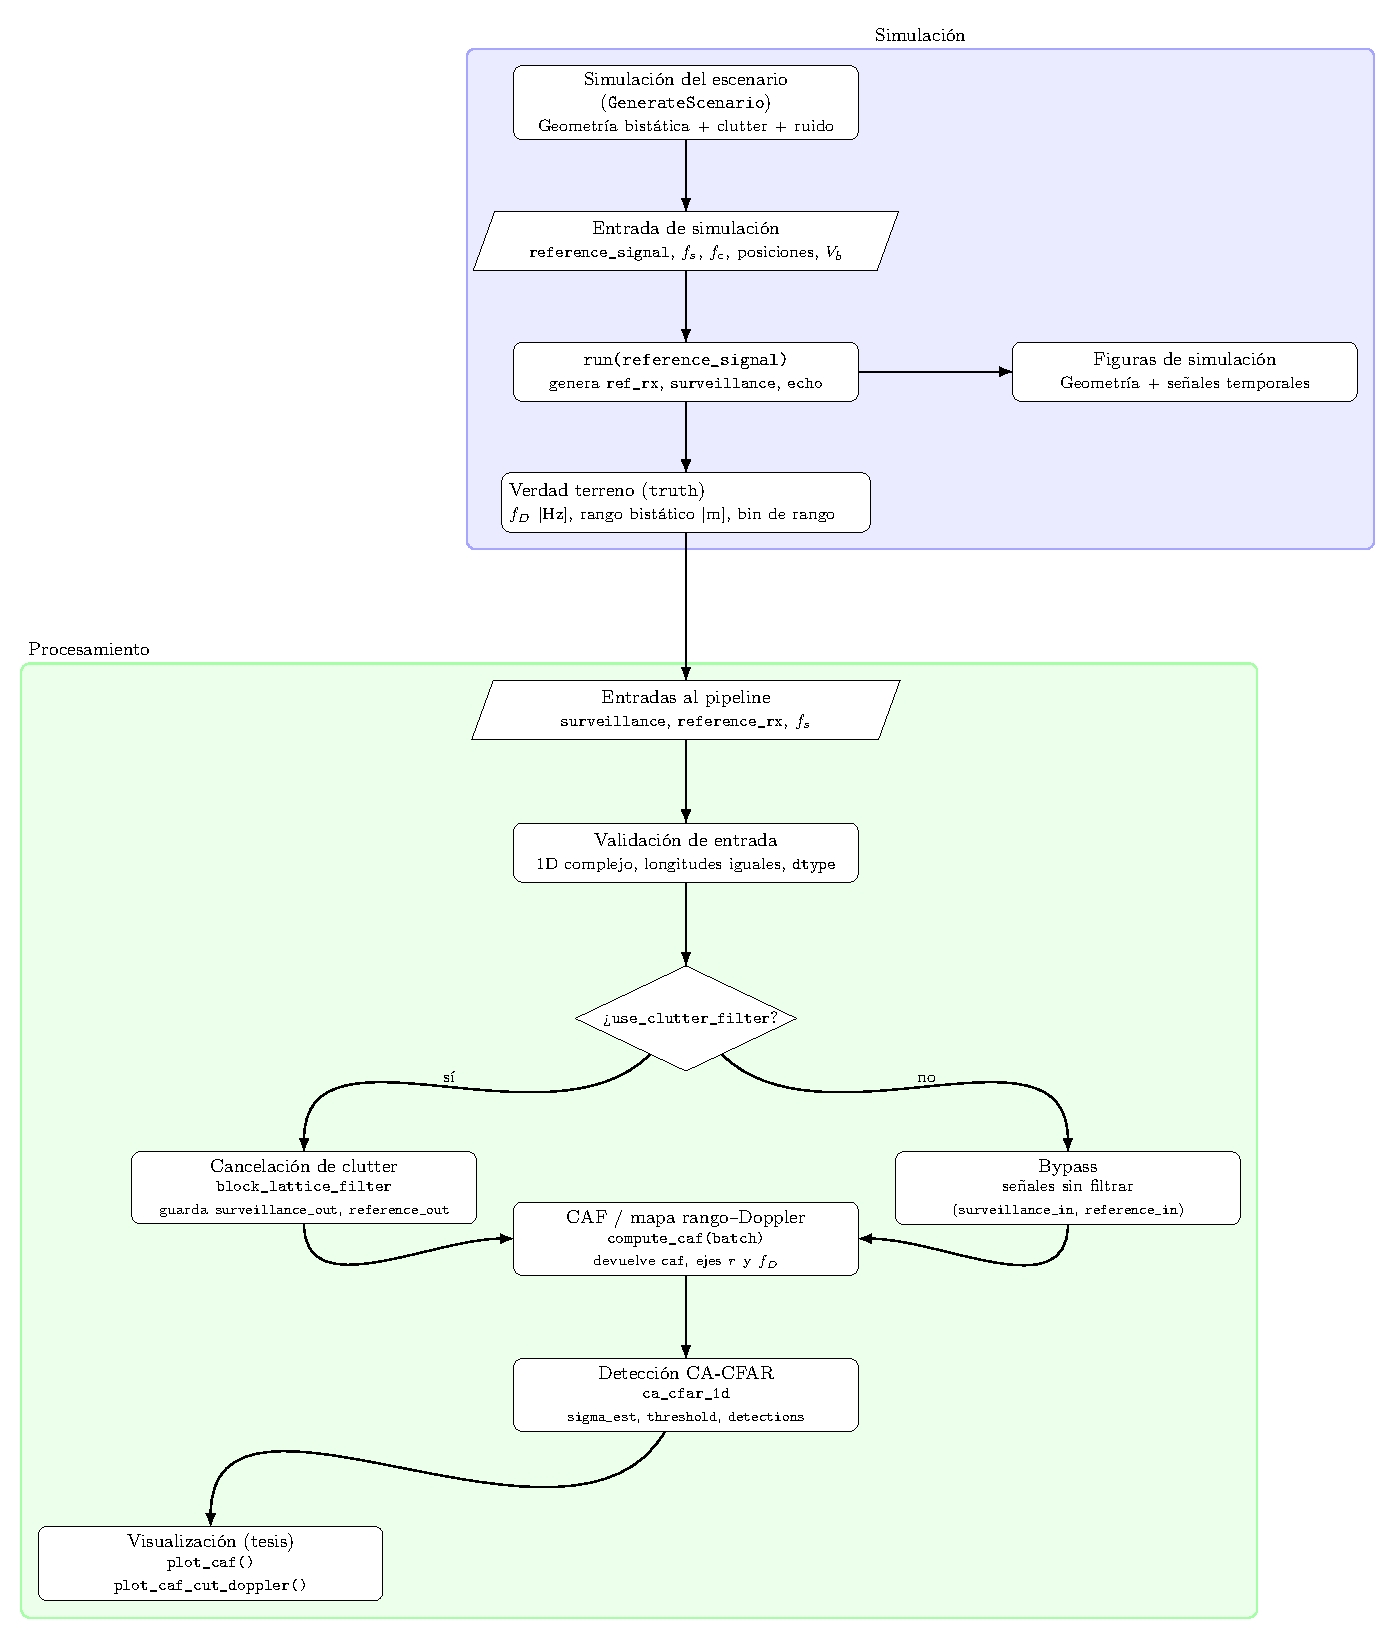
\includegraphics[width=0.85\textwidth]{pr/flow_pipeline_sim.pdf}
	\caption{Diagrama de flujo del proceso de simulación y procesamiento.}
	\label{fig:flow_pipeline_sim}
\end{figure}

\section{Escenario de simulación}

El escenario considerado consiste en un sistema de radar pasivo bistático con un transmisor fijo, un receptor fijo y un blanco en movimiento. Además, se incorporan múltiples reflectores estacionarios distribuidos en el entorno para modelar el clutter.

La Figura~\ref{fig:geometry_sim} muestra la geometría del escenario simulado.

\begin{figure}[H]
	\centering
	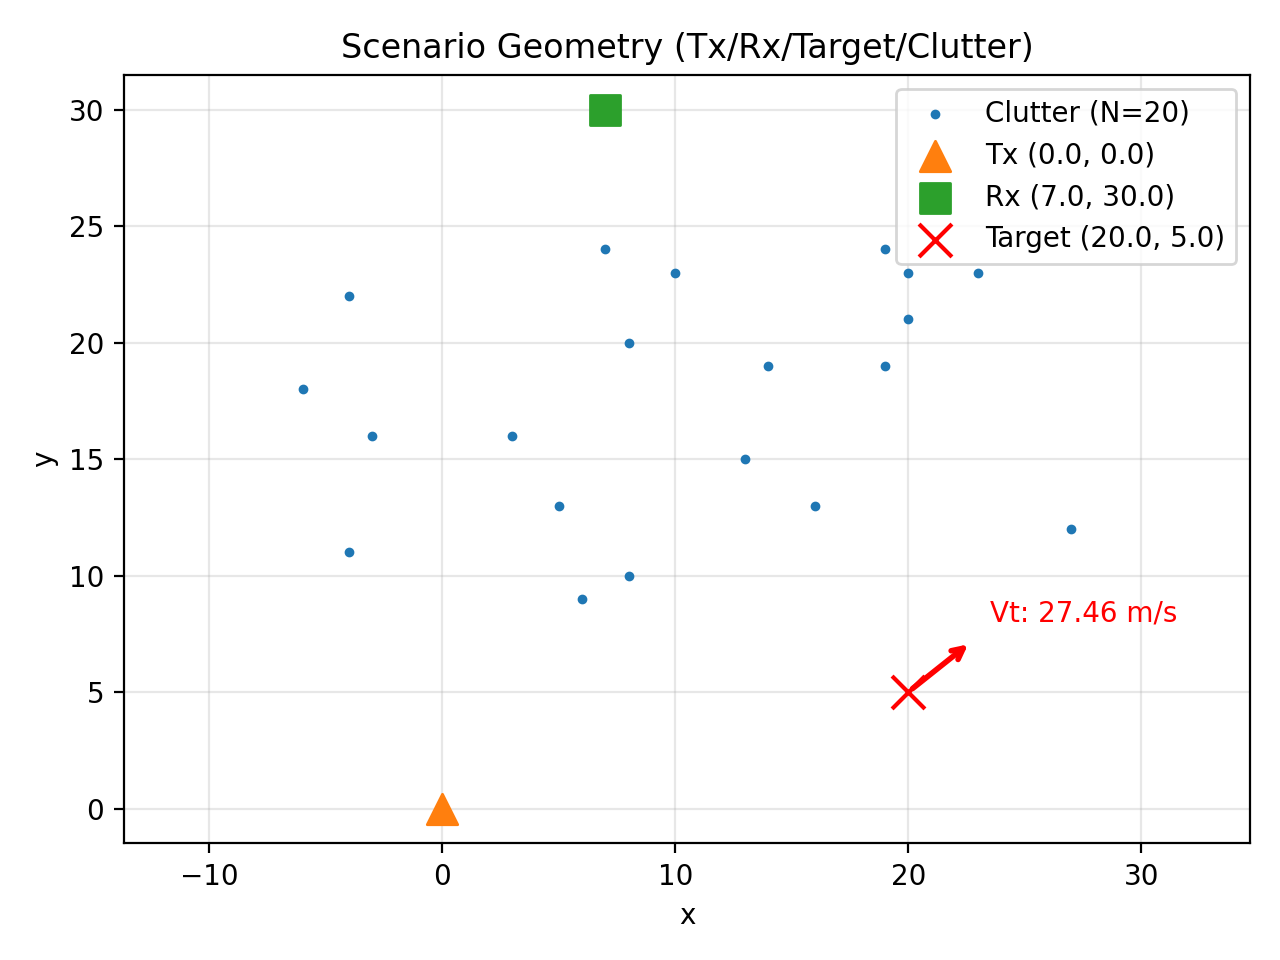
\includegraphics[width=0.6\textwidth]{sim_data/fig01_geometry.png}
	\caption{Geometría del escenario de simulación.}
	\label{fig:geometry_sim}
\end{figure}

A partir de esta configuración geométrica se generan las señales de referencia y vigilancia. La señal de vigilancia incluye la contribución del eco del blanco, la trayectoria directa del transmisor, múltiples reflexiones estacionarias y ruido aditivo.

El simulador devuelve, además, los valores de referencia del blanco (``ground truth''), en particular el rango bistático y el corrimiento Doppler esperados. Estos valores se utilizan posteriormente para validar la detección obtenida mediante la CAF y el detector CFAR.

\section{Análisis espectral de las señales}

Antes de aplicar la cadena de procesamiento, resulta útil analizar el contenido espectral de las señales generadas. Para ello se calcula la densidad espectral de potencia (PSD) utilizando el estimador implementado en el método \texttt{plot\_psd} del pipeline.

La Figura~\ref{fig:psd_input} muestra la PSD de las señales de entrada al sistema, es decir, el canal de referencia y el canal de vigilancia.

\begin{figure}[H]
	\centering
	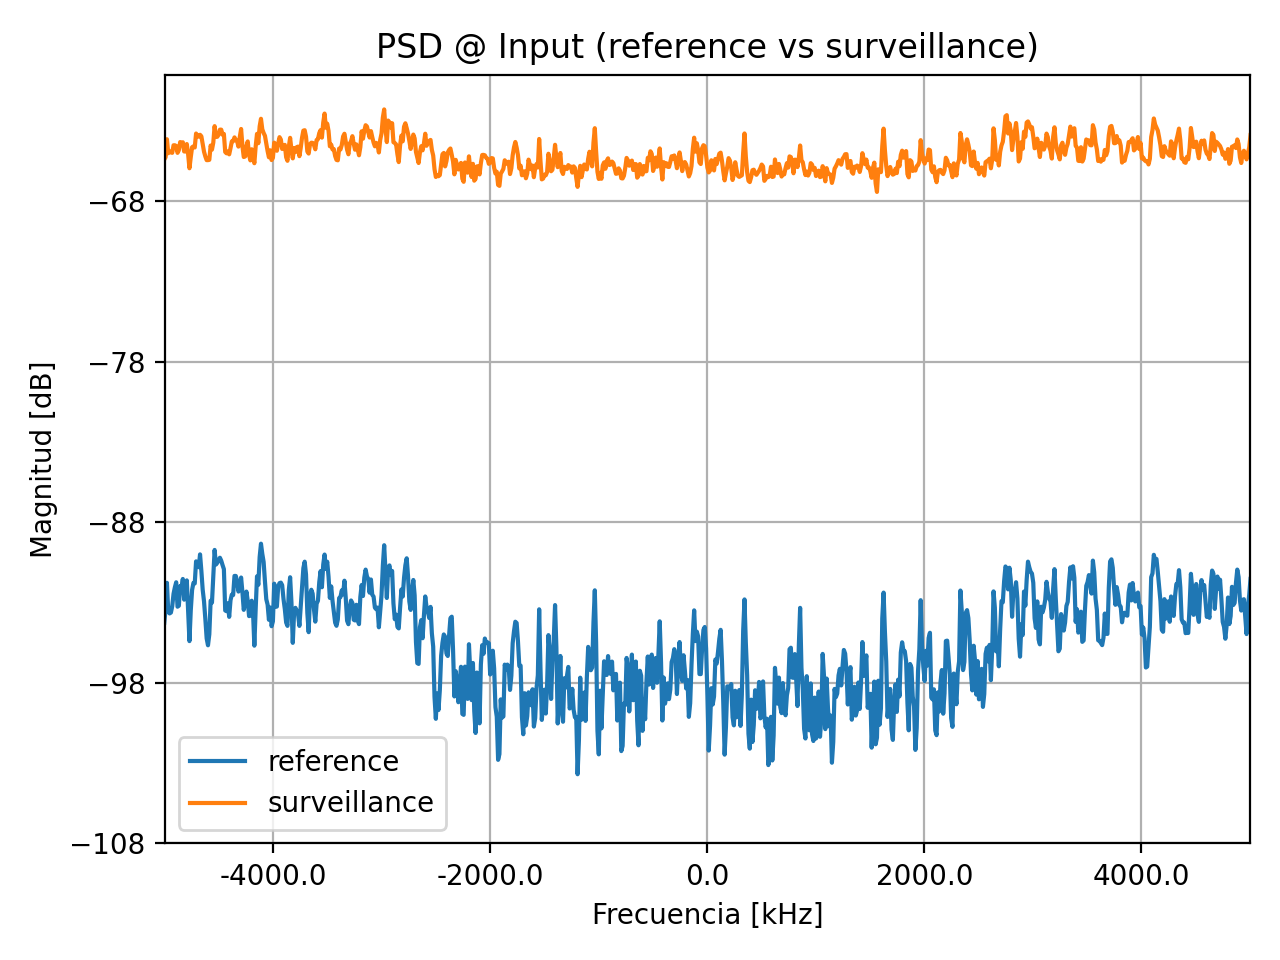
\includegraphics[width=0.8\textwidth]{sim_data/fig02_psd_input.png}
	\caption{PSD de las señales de entrada al pipeline.}
	\label{fig:psd_input}
\end{figure}

Puede observarse que ambas señales comparten el mismo ancho de banda, ya que la señal de vigilancia contiene copias retardadas y escaladas de la señal de referencia. Sin embargo, el canal de vigilancia presenta mayor potencia debido a la presencia de la trayectoria directa y del clutter, componentes altamente correlacionados con la referencia.

Este comportamiento es consistente con el modelo de señal presentado en el capítulo anterior, donde la interferencia de trayectoria directa y el clutter dominan la energía de la señal recibida.

\section{Efecto del filtro de clutter}

El siguiente paso consiste en aplicar el filtro adaptativo \textit{block lattice} para cancelar la trayectoria directa y las reflexiones estacionarias.

La Figura~\ref{fig:psd_caf_in} muestra la PSD de las señales que ingresan al bloque de cálculo de la CAF, es decir, la referencia y la señal de vigilancia luego del filtrado de clutter.

\begin{figure}[H]
	\centering
	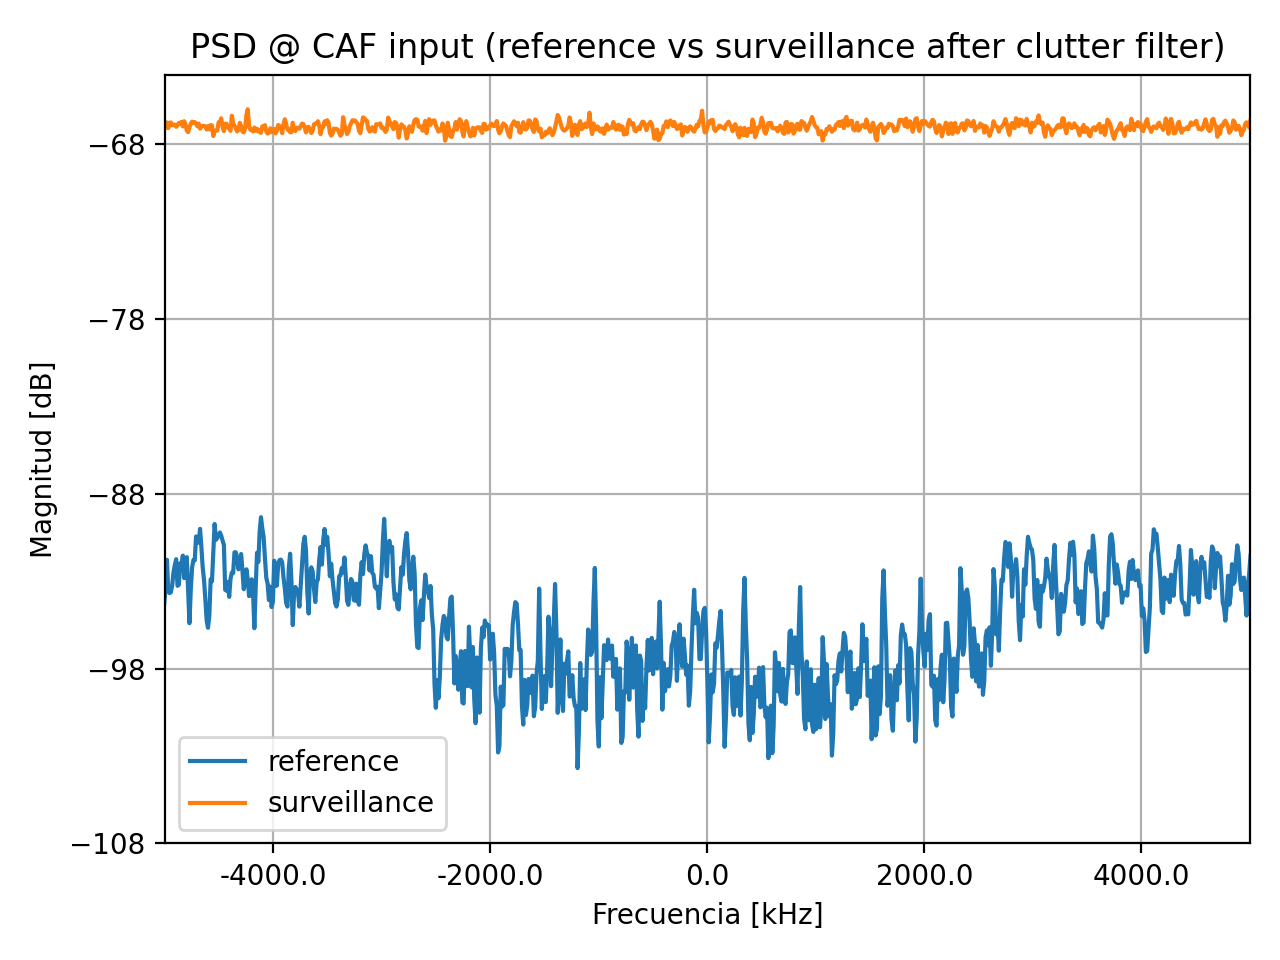
\includegraphics[width=0.8\textwidth]{sim_data/fig03_psd_caf_in.png}
	\caption{PSD a la entrada del bloque CAF luego del filtrado de clutter.}
	\label{fig:psd_caf_in}
\end{figure}

Se observa una reducción significativa de la potencia asociada a las componentes correlacionadas con la referencia, mientras que el ancho de banda de la señal se mantiene inalterado. Este comportamiento es el esperado para un filtro adaptativo de cancelación de clutter, cuyo objetivo es eliminar únicamente las componentes correlacionadas con la señal de referencia sin distorsionar la información restante.

Desde un punto de vista geométrico, este resultado refleja el proceso de proyección ortogonal descrito en la sección del filtro lattice: las componentes asociadas al subespacio generado por las copias retardadas de la referencia son removidas, preservando las componentes no correlacionadas, entre ellas los ecos de blancos en movimiento.

\section{Función de ambigüedad cruzada}

Una vez filtrada la señal de vigilancia, se calcula la función de ambigüedad cruzada mediante el algoritmo \textit{batch}. Este proceso produce un mapa rango--Doppler en el cual los blancos se manifiestan como máximos locales.

La Figura~\ref{fig:caf_no_cf} muestra la CAF obtenida sin aplicar el filtro de clutter.

\begin{figure}[H]
	\centering
	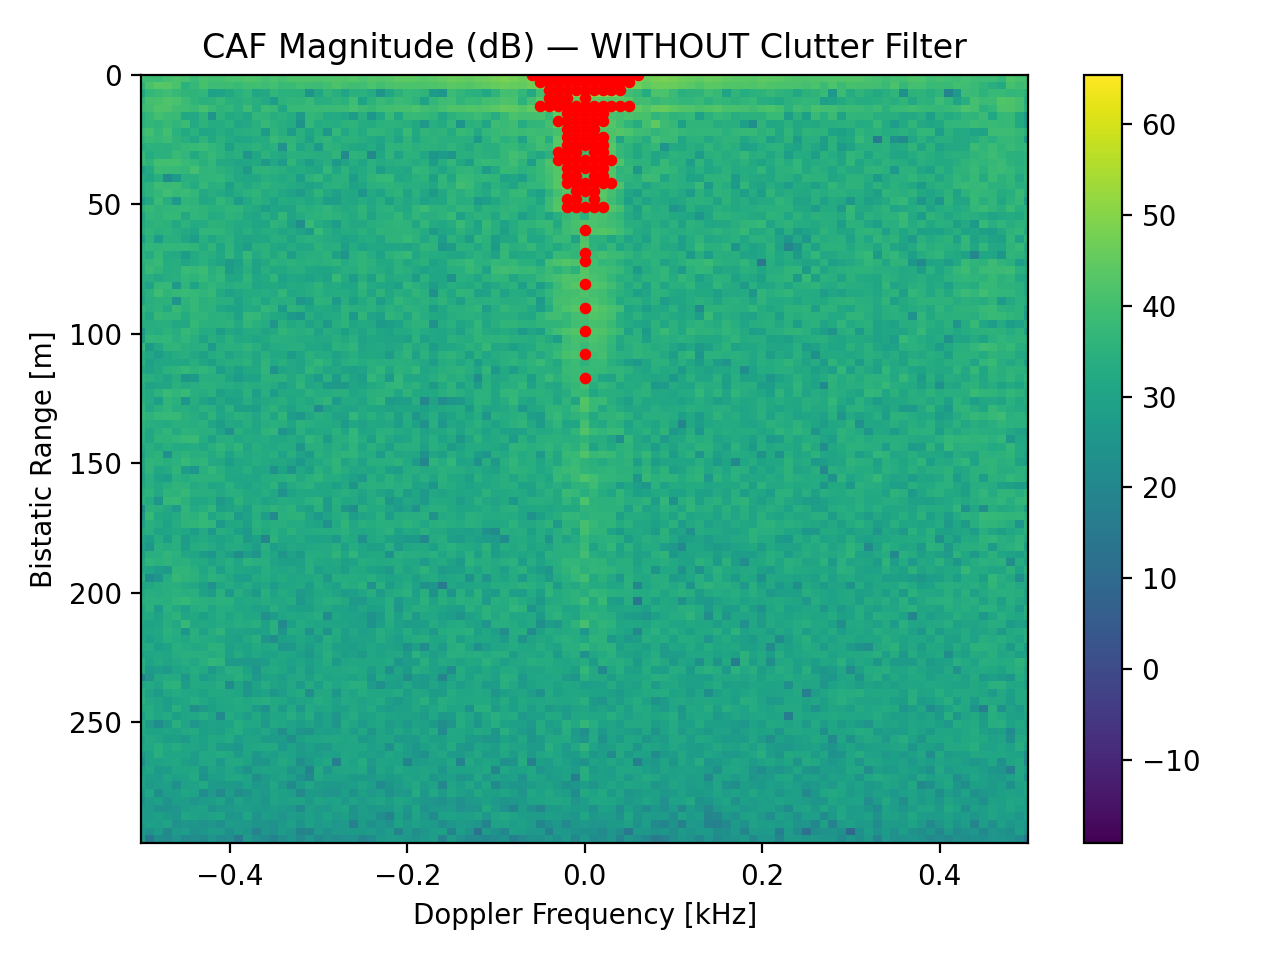
\includegraphics[width=0.8\textwidth]{sim_data/fig04_caf_no_clutter_filter.png}
	\caption{CAF sin filtrado de clutter.}
	\label{fig:caf_no_cf}
\end{figure}

En este caso, la presencia de la trayectoria directa y del clutter genera un nivel elevado de energía alrededor del origen Doppler, lo cual dificulta la identificación del blanco.

La Figura~\ref{fig:caf_cf} muestra la CAF obtenida luego de aplicar el filtro de clutter.

\begin{figure}[H]
	\centering
	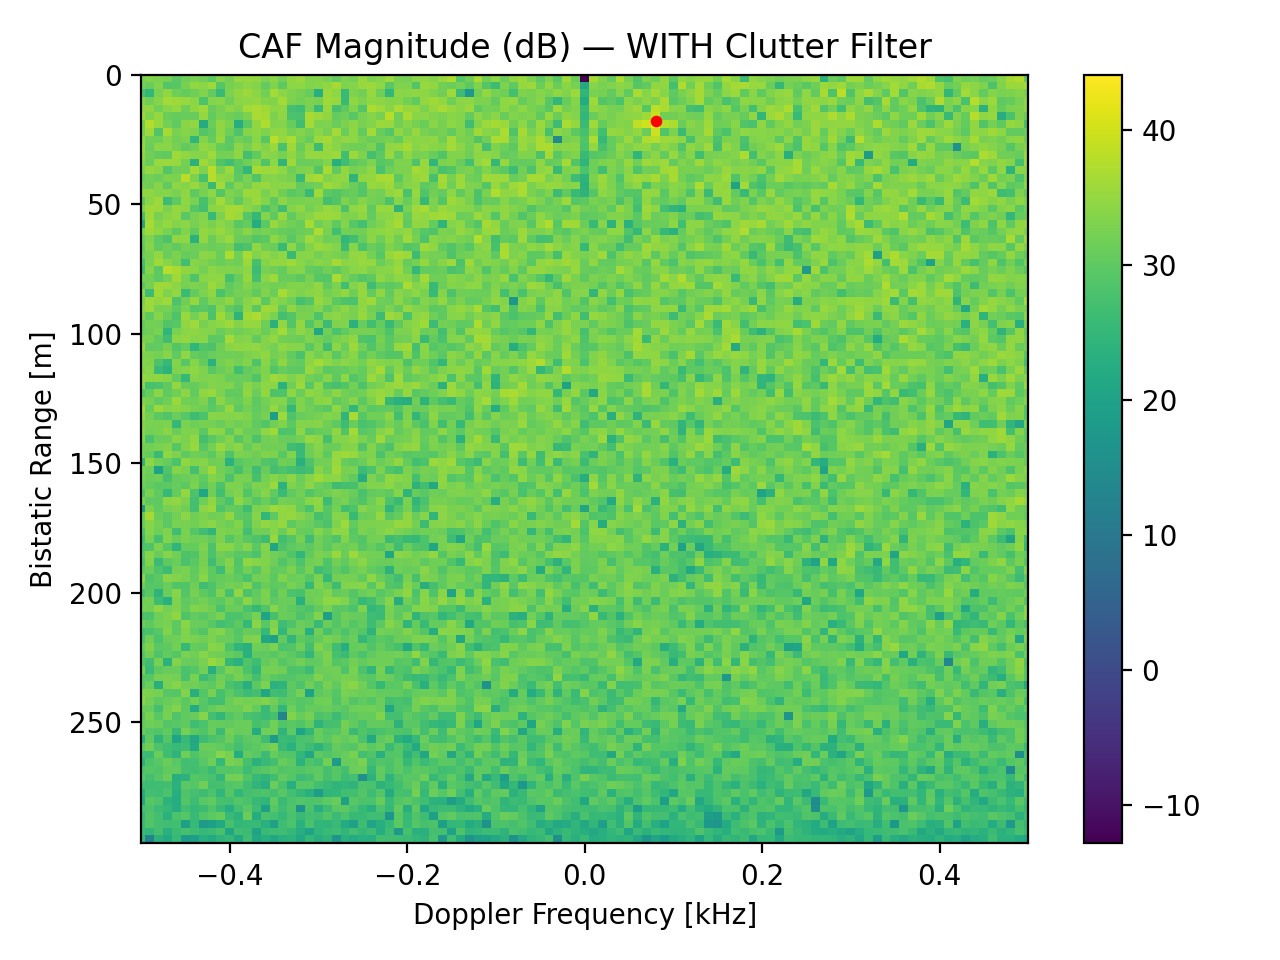
\includegraphics[width=0.8\textwidth]{sim_data/fig05_caf_with_clutter_filter.png}
	\caption{CAF luego del filtrado de clutter.}
	\label{fig:caf_cf}
\end{figure}

Puede observarse una mejora significativa en el contraste del mapa rango--Doppler, lo cual permite identificar con mayor claridad el eco del blanco. Este resultado confirma la utilidad del filtrado adaptativo para aumentar el rango dinámico efectivo del sistema.

\section{Detección mediante CFAR}

La detección de blancos se realiza aplicando el detector CA-CFAR sobre la magnitud de la CAF. Para analizar el comportamiento del detector, se considera un corte Doppler en el bin de rango correspondiente al blanco simulado.

La Figura~\ref{fig:cut_no_cf} muestra este corte sin filtrado de clutter, mientras que la Figura~\ref{fig:cut_cf} muestra el resultado luego del filtrado.

\begin{figure}[H]
	\centering
	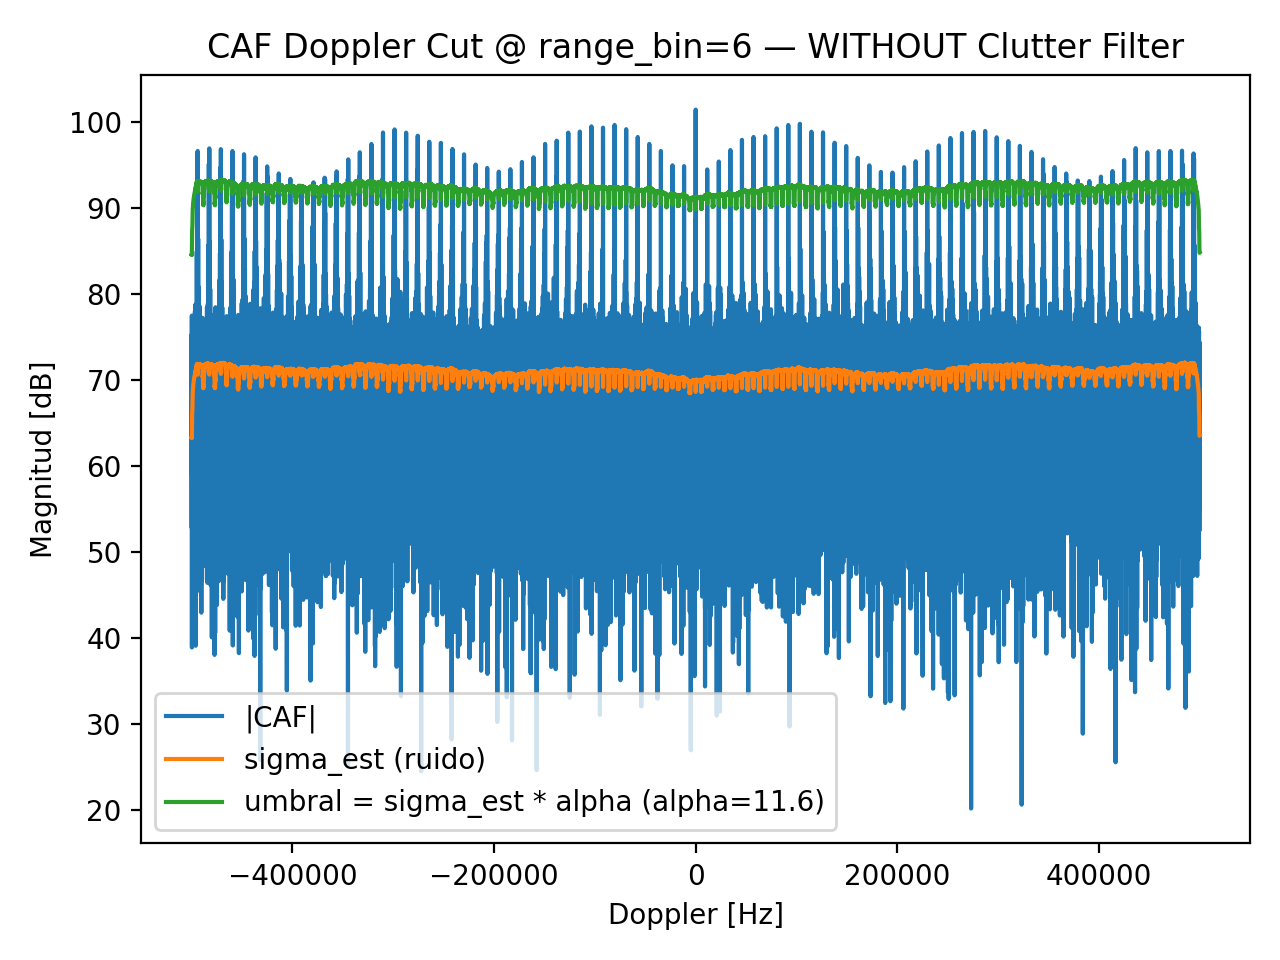
\includegraphics[width=0.8\textwidth]{sim_data/fig06_cut_no_clutter_filter.png}
	\caption{Corte Doppler sin filtrado de clutter.}
	\label{fig:cut_no_cf}
\end{figure}

\begin{figure}[H]
	\centering
	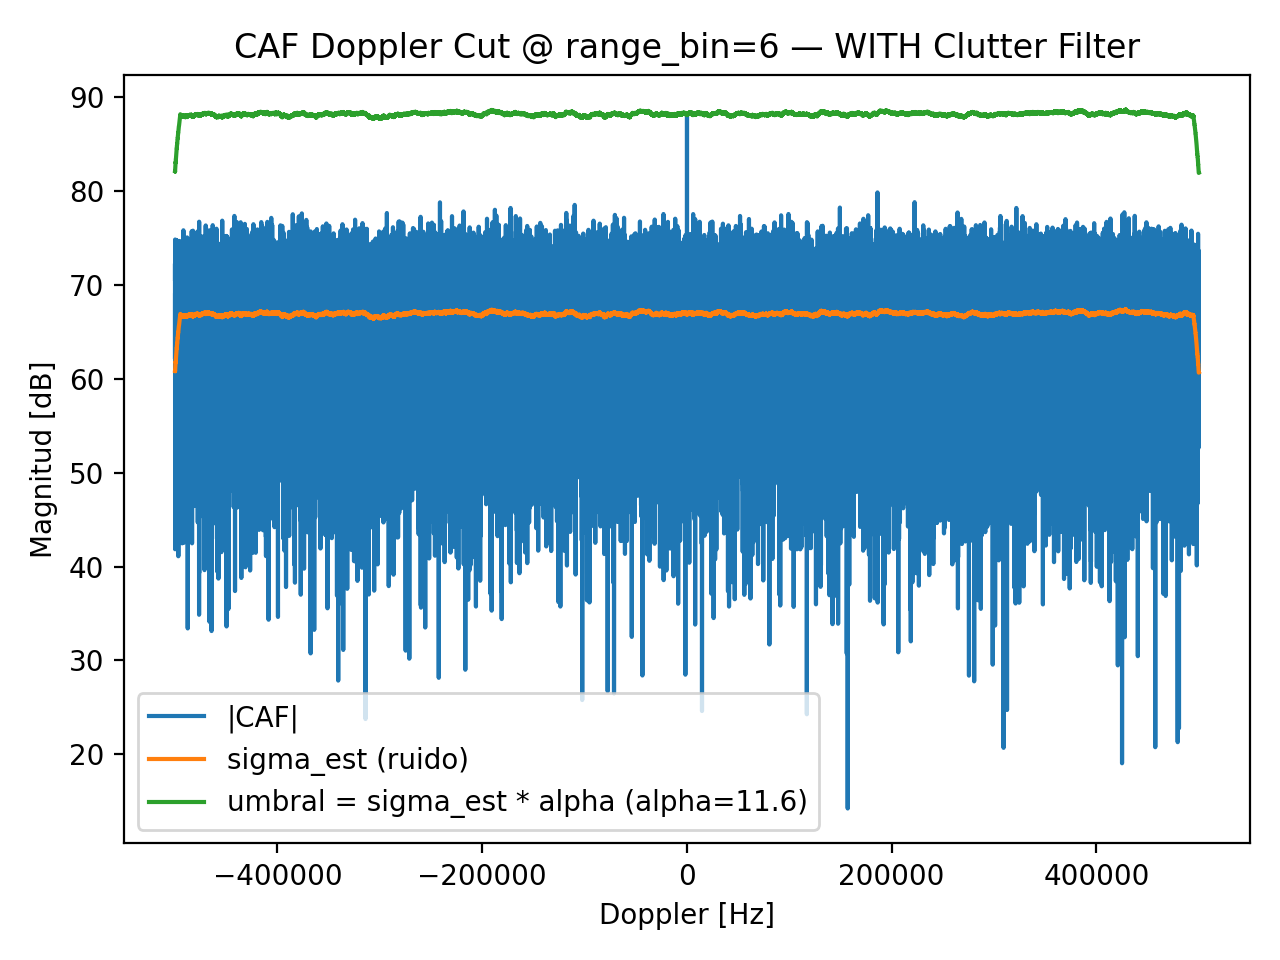
\includegraphics[width=0.8\textwidth]{sim_data/fig07_cut_with_clutter_filter.png}
	\caption{Corte Doppler luego del filtrado de clutter.}
	\label{fig:cut_cf}
\end{figure}

En el caso filtrado, el pico correspondiente al blanco supera claramente el umbral de detección estimado por el algoritmo CFAR. Este comportamiento es consistente con la teoría presentada en el capítulo anterior: al reducir la potencia del clutter, la estimación local del ruido disminuye y el detector puede operar con mayor sensibilidad.

\section{Validación}

La posición del máximo detectado en la CAF coincide con los valores de rango bistático y frecuencia Doppler calculados por el simulador. Esto confirma la correcta implementación de la cadena de procesamiento completa.

En conjunto, los resultados obtenidos validan el funcionamiento del sistema de radar pasivo simulado y muestran la importancia del filtrado de clutter para mejorar la detectabilidad de blancos en escenarios con interferencias dominantes.

	\chapter{Conclusiones}

En este trabajo se analizó el uso de la señal ISDB-Tb como iluminador de oportunidad en un sistema de radar pasivo biestático. Con ese objetivo, se estudió la estructura del estándar y, a partir de ello, se desarrolló una cadena de procesamiento.

A partir de las simulaciones realizadas, se observó que con la reconstrucción de la referencia se obtiene una mejora en el desempeño de la cadena, ya que se obtuvo una reducción entre 3 y 4 dB en el piso de ruido en el bloque de detección, cabe aclarar que las aproximaciones dependen directamente de las configuraciones del bloque CFAR y del bloque de ventaneo por lo que pueden variar para un mismo escenario y señal. En este sentido, esto se refleja en una mayor sensibilidad y en mejores condiciones para la detección de blancos.

Sin embargo, también se notó que con la mejora de ruido también se hicieron más evidentes ciertas componentes determinísticas dadas por el carácter cíclico y periódico de la señal. Esto no necesariamente invalida la utilización de este enfoque, simplemente hace notoria la necesidad de un postprocesamiento para limitar las detecciones espurias.

Con esto, se considera que se cumplieron los objetivos planteados al inicio del trabajo, ya que se logró analizar el estándar ISDB-Tb con el nivel de detalle correcto para el contexto y, por otro, se desarrolló una cadena de procesamiento completa que permitió analizar, en un entorno controlado, el efecto de reconstruir la señal de referencia sobre el desempeño del sistema.

\section{Trabajo futuro}

Las posibles mejoras y adiciones para continuar el trabajo presentado es que excedieron el marco del mismo, son la validación de la cadena utilizando señales reales para poder incorporar de manera más realista los efectos del canal, errores de sincronización y otras perturbaciones que no fueron contempladas en el modelo utilizado. También sería conveniente seguir con el análisis de la mitigación de las componentes determinísticas con estrategias como la del filtro recíproco.



	\appendix
	\cleardoublepage
	\phantomsection
	\addtocontents{toc}{\protect\contentsline{part}{Apéndices}{}{}}

	\chapter{Documentación de la cadena de procesamiento}
\label{ap:documentacion_codigo}

El presente apéndice documenta la implementación de software desarrollada para este trabajo. Su objetivo es complementar la descripción teórica de la cadena propuesta con una visión orientada a desarrolladores, de manera de dejar asentada la organización interna del código, su flujo de ejecución y los principales criterios adoptados para su extensión y reutilización. El contenido de esta sección se basa en la estructura actual del repositorio \texttt{PassiveRadarChain}, en la interfaz pública expuesta por el paquete y en la organización de sus módulos principales \cite{github-repo}.

\section{Objetivo del software}

La implementación busca materializar en código la cadena de procesamiento presentada en esta tesis. En particular, el repositorio está orientado a:

\begin{itemize}
    \item generar señales simuladas de referencia y vigilancia;
    \item cargar señales externas;
    \item aplicar una etapa opcional de canal y ruido;
    \item filtrar clutter y componente de señal directa;
    \item aplicar ventaneo sobre la referencia;
    \item calcular la función de ambigüedad cruzada;
    \item ejecutar detección CA-CFAR;
    \item facilitar ensayos comparativos y \textit{benchmarking} mediante reejecución parcial y acceso eficiente al estado interno.
\end{itemize}

De esta forma, el software no se limita a una colección de funciones aisladas, sino que provee una cadena integrada y reutilizable para simulación, procesamiento, validación y comparación sistemática de configuraciones.

\section{Organización general del repositorio}

A nivel superior, el repositorio se organiza en directorios destinados a datos, ejemplos, scripts y código fuente, además de los archivos auxiliares de instalación y configuración. El núcleo funcional del proyecto reside en el paquete \texttt{pr\_chain}, donde se concentra la implementación principal de la cadena.

Dentro del paquete, la organización actual se divide en cuatro submódulos principales:

\begin{itemize}
    \item \texttt{core}: contiene la clase principal de alto nivel y las dataclasses de configuración y estado;
    \item \texttt{processing}: agrupa los bloques algorítmicos de procesamiento radar;
    \item \texttt{generators}: contiene los generadores de eco y clutter para simulación;
    \item \texttt{utils}: incluye constantes, utilidades matemáticas y funciones de graficado.
\end{itemize}

Esta separación responde a un criterio funcional: por un lado, desacopla la lógica de orquestación de la cadena respecto de los algoritmos individuales; por otro, distingue con claridad los bloques de simulación, los bloques de procesamiento y las herramientas auxiliares.

\section{API pública del paquete}

El punto de entrada del paquete expone de manera directa los componentes más importantes para el usuario o desarrollador. En particular, \texttt{pr\_chain} reexporta la clase principal de la cadena, las funciones de procesamiento más relevantes, los generadores de clutter y eco, y los submódulos utilitarios asociados.

Esto permite trabajar tanto a nivel de cadena completa como a nivel de bloques individuales, según convenga al tipo de experimento que se quiera realizar. En otras palabras, el diseño no obliga a utilizar siempre la abstracción de más alto nivel, sino que conserva la posibilidad de reutilizar funciones y clases por separado.

En la versión actual, la interfaz pública de \texttt{PassiveRadarChain} se apoya en tres ideas complementarias. La primera es ofrecer métodos de alto nivel para configurar y ejecutar la cadena completa. La segunda es permitir el acceso a estados intermedios de manera controlada. La tercera es mantener compatibilidad hacia atrás mediante métodos específicos de actualización de configuración, aun cuando internamente exista una interfaz más general para modificar distintas secciones de la configuración.

\section{Arquitectura central: \texttt{PassiveRadarChain}}

La pieza principal del repositorio es la clase \texttt{PassiveRadarChain}, ubicada en el submódulo \texttt{core}. Esta clase implementa una cadena de procesamiento con estado, pensada para operar sobre señales reales o simuladas, almacenar resultados intermedios y permitir la reejecución parcial de etapas sin recalcular innecesariamente toda la secuencia de procesamiento.

La cadena se organiza internamente según el siguiente orden de etapas:

\begin{equation*}
\texttt{inputs} \rightarrow
\texttt{channel} \rightarrow
\texttt{filter} \rightarrow
\texttt{window} \rightarrow
\texttt{caf} \rightarrow
\texttt{detect}.
\end{equation*}

Cada una de estas etapas puede ejecutarse de forma individual o como parte de una corrida completa. Además, la clase provee métodos de alto nivel para correr la cadena completa, correrla desde una etapa dada, detenerla en una etapa intermedia y decidir si el estado devuelto debe copiarse en profundidad o devolverse como referencia directa al estado interno.

Este último punto resulta especialmente relevante en escenarios de \textit{benchmarking}. En ejecuciones repetidas, la copia profunda de estructuras grandes ---por ejemplo, matrices CAF o estimaciones bidimensionales del nivel de ruido--- puede introducir un costo extra que no forma parte del procesamiento radar en sí. Por este motivo, la implementación actual permite desactivar esa copia cuando se busca maximizar la eficiencia en estudios comparativos.

\section{Modelo de configuración}

La configuración del sistema se implementa mediante una jerarquía de dataclasses agrupadas en una configuración principal de la cadena. Esta clase principal encapsula subconfiguraciones para entrada, canal, simulación, ventaneo, filtrado, CAF, CFAR, graficado y entrada/salida.

En particular, las configuraciones más importantes son:

\begin{itemize}
    \item configuración de entrada: frecuencia de muestreo, frecuencia portadora, longitud de señal y selección entre entradas reales o simuladas;
    \item configuración de canal: habilitación de canal, agregado de ruido, potencia de ruido, respuesta de canal y decisión de agregar ruido a uno o ambos canales;
    \item configuración de simulación: geometría del escenario, presencia de señal directa y subconfiguraciones de clutter y eco;
    \item configuración de ventana: habilitación del ventaneo y parámetros de la ventana de Kaiser;
    \item configuración de filtro: habilitación y orden del filtro lattice;
    \item configuración de CAF: tamaño de bloque del cálculo \textit{batch};
    \item configuración de CFAR: dimensionalidad del detector, celdas de entrenamiento, celdas de guarda, probabilidad de falsa alarma y tratamiento periódico del eje Doppler;
    \item configuración de graficado: parámetros de visualización;
    \item configuración de entrada/salida: rutas y formato de salida.
\end{itemize}

Un aspecto importante del diseño es que estas dataclasses no cumplen únicamente el rol de contenedores de parámetros. Varias de ellas incorporan validaciones y normalización en sus métodos de inicialización, lo que ayuda a detectar errores de configuración en etapas tempranas y vuelve más robusta la interacción con archivos serializados o con parámetros cargados dinámicamente.

En la versión refactorizada, la actualización de parámetros puede realizarse mediante una interfaz general que identifica la sección de configuración a modificar, mientras que se conservan métodos específicos del tipo \texttt{update\_input\_config()}, \texttt{update\_filter\_config()} o \texttt{update\_cfar\_config()} para preservar compatibilidad y claridad de uso. De esta manera, el código de usuario puede seguir invocando la API previa, pero la lógica interna de actualización e invalidación queda centralizada.

\section{Modelo de estado}

Además de la configuración, la cadena mantiene un estado de ejecución explícito mediante un conjunto de dataclasses de estado. Estas estructuras almacenan el resultado de una etapa particular, mientras que un contenedor de estado global reúne la información total de la cadena, incluyendo resultados intermedios, etapas completadas, \textit{snapshots} de configuración y la última etapa ejecutada.

Este esquema tiene dos ventajas principales. En primer lugar, facilita la inspección del procesamiento en puntos intermedios, lo cual es especialmente útil durante tareas de depuración, comparación y análisis de resultados. En segundo lugar, permite invalidar selectivamente etapas y conservar resultados previos cuando los cambios de configuración no afectan a toda la cadena.

La versión actual distingue además entre dos formas de acceso al estado. La primera devuelve una copia profunda de la estructura solicitada, lo cual resulta más seguro para uso interactivo. La segunda devuelve una referencia directa al estado interno, evitando copias de arreglos grandes y favoreciendo estudios de rendimiento. Esta separación permite mantener una API cómoda para exploración general y, al mismo tiempo, una vía eficiente para experimentos repetitivos.

\section{Estrategia de ejecución e invalidación}

Uno de los aspectos más importantes de la implementación es la presencia de un mecanismo de \textit{cache} e invalidación automática basado en \textit{snapshots} de configuración. La clase construye, para cada etapa, una versión serializable de la configuración relevante y la compara con la utilizada en la última ejecución. Si detecta cambios, invalida esa etapa y las posteriores.

Desde el punto de vista del desarrollo, esto vuelve a la cadena particularmente cómoda para experimentación iterativa. Por ejemplo, si únicamente cambia la configuración del detector CFAR, no es necesario regenerar señales, volver a aplicar canal, recalcular el filtrado ni reconstruir la CAF desde cero. Del mismo modo, si cambia la configuración de simulación, la invalidación se propaga desde la etapa de entrada.

En la versión refactorizada, esta misma lógica también contempla la posibilidad de modificar la señal de referencia que ingresa a la CAF. Si se activa una referencia reconstruida, la invalidación se propaga desde la etapa \texttt{caf}, sin necesidad de recalcular las etapas anteriores. Esto resulta especialmente útil cuando se desea comparar, sobre una misma señal de vigilancia, el desempeño de la referencia original frente a distintas estrategias de reconstrucción.

\section{Etapas funcionales de la cadena}

\subsection{Entradas y simulación}

La cadena admite dos modos de trabajo. En el primero, el usuario provee directamente las señales de referencia y vigilancia o las carga desde archivo. En el segundo, la propia cadena genera entradas simuladas a partir de la configuración del escenario.

Cuando se trabaja en modo simulado, la referencia se genera como una señal compleja y luego se construyen el clutter y el eco mediante clases específicas. El canal de vigilancia se obtiene combinando clutter, eco y, opcionalmente, la señal directa.

La implementación actual también verifica la consistencia entre las señales de entrada y una eventual referencia reconstruida definida para la CAF. Si la longitud de las señales cambia y el reemplazo deja de ser compatible, dicho reemplazo se invalida automáticamente para evitar inconsistencias internas.

\subsection{Canal y ruido}

La etapa de canal es opcional y permite aplicar una respuesta de canal común a referencia y vigilancia, así como agregar ruido blanco gaussiano aditivo. Esta separación resulta útil porque desacopla el problema de simulación geométrica del problema de degradación del canal. En otras palabras, la escena radar y las imperfecciones del sistema pueden modelarse de manera independiente.

Además, la configuración permite decidir si el ruido se agrega solamente a vigilancia o a ambos canales, lo cual resulta conveniente cuando se busca aproximar distintos esquemas de recepción o aislar el efecto de determinadas degradaciones.

\subsection{Filtrado de clutter}

La etapa de filtrado implementa un filtro lattice por bloques para atenuar clutter y componente de camino directo en la señal de vigilancia. El parámetro principal del bloque es el orden del filtro, entendido como la cantidad de etapas de cancelación aplicadas.

Este diseño condensa en un bloque reutilizable la etapa anti-clutter presentada en el cuerpo principal de la tesis, y permite explorar directamente cómo cambia la salida del sistema al modificar el orden del filtro.

\subsection{Ventaneo}

La etapa de ventaneo aplica una ventana de Kaiser a la señal de referencia. La implementación admite ventaneo en frecuencia, en rango o en ambos dominios, y acepta tanto un único parámetro $\beta$ como una tupla con valores diferenciados para cada operación.

Desde el punto de vista experimental, este diseño resulta valioso porque habilita el estudio del compromiso entre supresión de lóbulos laterales y degradación de resolución sin alterar el resto de la cadena.

\subsection{CAF}

El cálculo de la CAF se realiza mediante un algoritmo \textit{batch}. La función correspondiente recibe el tamaño de bloque, la frecuencia de muestreo y las señales de referencia y vigilancia, y devuelve la matriz CAF junto con sus ejes de frecuencia Doppler y rango.

En la operación habitual, la referencia utilizada en esta etapa es la salida del bloque de ventaneo. Sin embargo, la versión actual de la cadena permite reemplazar esa entrada por una señal de referencia reconstruida definida explícitamente por el usuario. Esta funcionalidad resulta útil, por ejemplo, cuando se desea evaluar el efecto de un reconstructor sobre la supresión del clutter, la compresión en rango o la calidad global del mapa rango--Doppler, manteniendo fijo el resto del procesamiento.

En la implementación actual, la CAF se calcula sobre señales truncadas a un múltiplo exacto del tamaño de bloque, y la etapa encapsulada en la clase también construye los parámetros auxiliares necesarios para visualización y análisis posterior. De este modo, la lógica de cálculo y la preparación de salidas para análisis permanecen integradas en un único bloque de alto nivel.

\subsection{Detección}

La etapa final implementa un detector CA-CFAR sobre la magnitud de la CAF. La implementación admite tanto detección unidimensional sobre frecuencia como detección bidimensional, y permite definir tamaños de ventana y guarda mediante enteros o tuplas.

La salida del detector incluye las detecciones, la estimación local del nivel de ruido o clutter y el factor de escala aplicado para construir el umbral de decisión.

\section{Módulos de simulación}

El paquete contiene generadores específicos para la construcción de escenarios simulados.

Por un lado, el generador de clutter modela múltiples reflectores estacionarios distribuidos en el plano. A partir de la geometría transmisor--clutter--receptor, calcula retardos biestáticos y construye la señal de clutter como suma de copias retardadas y escaladas de la referencia.

Por otro lado, el generador de eco modela un blanco puntual en movimiento. A partir de la geometría transmisor--blanco--receptor y del vector velocidad del objetivo, calcula el retardo biestático y la frecuencia Doppler asociada, y construye la señal de eco como una copia retardada, modulada en fase y escalada de la referencia.

Estas clases resultan particularmente valiosas desde el punto de vista del desarrollo, ya que permiten desacoplar la validación algorítmica de la disponibilidad de señales reales y construir escenarios controlados donde la verdad de terreno es conocida.

\section{Utilidades auxiliares}

El submódulo \texttt{utils} reúne componentes de apoyo que simplifican el uso del paquete. Allí se incluyen constantes físicas, utilidades matemáticas y funciones de graficado.

Estas utilidades no forman parte del núcleo lógico de la cadena, pero cumplen un rol importante en la reproducibilidad y en la interpretación de resultados, ya que estandarizan tanto ciertas operaciones numéricas como la forma de visualización.

En particular, las utilidades de graficado se integran con la clase principal para visualizar la geometría del escenario, la CAF y las detecciones estimadas, así como para guardar figuras dentro del árbol de salida definido por la configuración del proyecto.

\section{Persistencia y salidas}

La clase principal resuelve un directorio raíz de salida y crea, si es necesario, subdirectorios para configuraciones, estados y figuras. Si el usuario no define explícitamente una ruta, la implementación utiliza por defecto un directorio de salida en el nivel superior del proyecto, con subcarpetas separadas para configuraciones, estados y figuras.

Este esquema resulta adecuado para preservar trazabilidad experimental, ya que facilita separar la lógica del código de los artefactos generados durante la ejecución.

La persistencia no se limita a la configuración global. La cadena permite serializar el estado numérico de ejecución, incluyendo señales intermedias, resultados de filtrado, CAF, detecciones y metadatos asociados a las etapas completadas. En la versión actual, esta persistencia también puede conservar información adicional asociada a la referencia reconstruida utilizada como entrada de la CAF, lo cual favorece la repetibilidad de ensayos comparativos.

\section{Flujo típico de uso}

Desde el punto de vista de un desarrollador, un flujo mínimo de trabajo con el paquete puede resumirse en los siguientes pasos:

\begin{enumerate}
    \item crear o modificar una configuración;
    \item instanciar la cadena principal;
    \item definir entradas reales o habilitar simulación;
    \item ejecutar la cadena completa o hasta una etapa intermedia;
    \item inspeccionar el estado devuelto o acceder al estado interno sin copias profundas si se busca eficiencia;
    \item modificar parámetros, cambiar la referencia de la CAF si corresponde y relanzar desde la etapa necesaria.
\end{enumerate}

Un ejemplo mínimo de uso podría escribirse como:

\begin{Verbatim}[breaklines=true, breakanywhere=true, fontsize=\small]
from pr_chain import PassiveRadarChain

chain = PassiveRadarChain()
chain.update_input_config(N=500_000, fs=8e6, f_c=700e6)
chain.update_filter_config(enabled=True, order=30)
chain.update_window_config(enabled=True, beta=(14.0, 14.0), freq=True, range=False)
chain.update_caf_config(batch=200)
chain.update_cfar_config(enabled=True, bidimensional=False, Nw=512, Ng=8, P_fa=1e-6)

state = chain.run(copy_state=False)
caf_state = chain.peek_state("caf")
det_state = chain.peek_state("detection")
\end{Verbatim}

En este ejemplo, la cadena utiliza el modo de simulación por defecto, ejecuta todas las etapas hasta detección y luego permite acceder tanto a la CAF como al estado del detector sin incurrir en copias profundas adicionales. Esta modalidad resulta apropiada en estudios repetitivos o comparaciones de rendimiento.

Si se dispone de una referencia reconstruida, esta puede utilizarse como entrada del bloque CAF mediante una interfaz explícita, por ejemplo:

\begin{Verbatim}[breaklines=true, breakanywhere=true, fontsize=\small]
chain.set_reconstructed_reference(reference_rec)
chain.run_from("caf", copy_state=False)
caf_state = chain.peek_state("caf")
\end{Verbatim}

En este segundo ejemplo, las etapas previas permanecen inalteradas y únicamente se recalculan la CAF y la detección a partir de la nueva referencia. La API también admite trabajar con entradas externas mediante los métodos de carga o asignación directa.

\section{Criterios de extensibilidad}

La arquitectura actual favorece varias formas de extensión.

La primera consiste en reemplazar o mejorar funciones individuales de procesamiento, por ejemplo incorporando nuevos esquemas de filtrado anti-clutter, otros algoritmos de cálculo de CAF o detectores alternativos a CA-CFAR. Como la clase principal orquesta estas funciones desde etapas bien definidas, las modificaciones pueden acotarse a un bloque sin necesidad de reescribir toda la cadena.

La segunda consiste en ampliar el subsistema de simulación, agregando nuevas fuentes de degradación, múltiples blancos o modelos geométricos más sofisticados. La existencia de clases separadas para eco y clutter facilita este camino.

La tercera consiste en extender la lógica de entrada a la etapa de CAF, incorporando nuevos reconstructores o métodos de síntesis de referencia sin alterar la estructura general de la cadena. La existencia de un punto explícito de reemplazo para esta referencia favorece ese tipo de experimentos.

La cuarta consiste en enriquecer la documentación y los ejemplos de uso. Si bien el repositorio ya incluye una estructura coherente de paquete, un archivo de instalación y documentación básica, una evolución natural del proyecto sería incorporar más ejemplos reproducibles, pruebas automatizadas y documentación generada a partir de docstrings.

\section{Observaciones finales}

Desde la perspectiva de esta tesis, la implementación de \texttt{pr\_chain} constituye más que un soporte instrumental para obtener resultados. En rigor, se trata de uno de los productos centrales del trabajo, ya que cristaliza en software la integración entre simulación, comprensión del problema radar y evaluación del impacto de distintas estrategias de procesamiento.

Por este motivo, entendemos que el valor del desarrollo no reside únicamente en el resultado numérico obtenido en los experimentos, sino también en haber dejado una base modular, legible y reutilizable, orientada a libre uso y suficientemente estructurada como para servir como punto de partida en extensiones futuras \cite{github-repo}.

	\chapter{Generación de señales, reconstrucción y procesamiento}
\section{GNU Radio}
Para generar la señal ISDB-Tb se utilizaron los bloques de procesamiento publicados en~\cite{grisdbt_repo}. A partir de estos bloques se construyeron los flujos de transmisión, recepción y remodulación mostrados en las Figuras~\ref{fig:isdbt_iluminador}--\ref{fig:tx_remod}.

\figura{\Tfig}{./gnu_radio/tx.png}{Generación de la señal ISDB-Tb del iluminador de oportunidad.}{}{\label{fig:isdbt_iluminador}}

\figura{\Tfig}{./gnu_radio/rx_A.png}{Recepción y demodulación de la referencia ruidosa (Capa A).}{}{\label{fig:rx_A}}
\figura{\Tfig}{./gnu_radio/rx_B.png}{Recepción y demodulación de la referencia ruidosa (Capa B).}{}{\label{fig:rx_B}}

\figura{\Tfig}{./gnu_radio/tx_remod.png}{Remodulación para obtener referencia reconstruida.}{}{\label{fig:tx_remod}}

La Figura~\ref{fig:isdbt_iluminador} muestra el flujo utilizado para generar la señal ISDB-Tb asociada al iluminador de oportunidad. Luego, las Figuras~\ref{fig:rx_A} y~\ref{fig:rx_B} presentan los flujos de recepción correspondientes a las capas A y B, respectivamente. Finalmente, la Figura~\ref{fig:tx_remod} muestra el flujo de remodulación empleado para obtener la referencia reconstruida, la cual será comparada con la referencia ruidosa en la cadena de procesamiento.

\newpage
\section{Implementación de las cadenas de procesamiento}
\subsection{Generación de canal de vigilancia y referencia}
El Listado~\ref{lst:gen_signals} presenta la función encargada de generar las señales utilizadas en la simulación. Esta función agrega ruido complejo a la señal ISDB-Tb de referencia y configura una escena de radar pasivo para obtener la referencia ruidosa y el canal de vigilancia que luego se usaran en la cadena de procesamiento.\\\vspace{5pt}
\begin{lstlisting}[
    style=pythoncompact,
    caption={Función para generar las señales de referencia y vigilancia simuladas.},
    label={lst:gen_signals}
]
def gen_signals(snr_db, reference, echo_power_db, samples=N_SAMPLES):
    N = len(reference)
    E_ref = np.mean(np.abs(reference) ** 2)
    noise_power = E_ref / utils.from_db(snr_db)
    noise = (
        np.sqrt(noise_power)
        * (np.random.randn(N) + 1j * np.random.randn(N))
    ).astype(np.complex64)

    noisy_ref = (reference + noise).astype(np.complex64)
    noisy_ref.tofile(DATA_DIR / "gr_files" / "isdbt_noisy.cfile")

    pr_config = PassiveRadarChainConfig(
        input=InputConfig(
            N=samples, fs=8126984.0, f_c=700e6, use_simulated_data=True
        ),
        simulation=SimulationConfig(
            transmitter_position=[0.0, 0.0],
            radar_position=[50.0, 500.0],
            direct_signal=True,
            clutter=ClutterConfig(
                N_CLUTT=10,
                clutter_rcs_min_db=-3.0,
                clutter_rcs_max_db=-5.0,
                rand_clutter=True,
                clutter_limits=[-100, 2000, 5, 150],
            ),
            echo=EchoConfig(
                V_b=[10.0, 100.0],
                rand_target=False,
                target_rcs_db=echo_power_db,
                target_position=[2500.0, 120.0],
            ),
        ),
        channel=ChannelConfig(
            enable=False,
        ))
    
    noise_surv = (
        np.sqrt(noise_power)
        * (np.random.randn(samples) + 1j * np.random.randn(samples))
    )

    pr_chain = PassiveRadarChain(pr_config)
    pr_chain.simulate_inputs(reference[:samples])    
    
    input_state= pr_chain.get_state(stage= "inputs", copy_state=False)
    sim_state = pr_chain.get_state(stage="simulation", copy_state=False)

    surv = input_state.surveillance + noise_surv
    fd, target_p = sim_state.doppler_hz, sim_state.target_position

    return noisy_ref[0:samples], surv, fd, target_p
\end{lstlisting}
\newpage
\subsection{Ejecución de la cadena de procesamiento}
El Listado~\ref{lst:run_config} muestra la función encargada de ejecutar la cadena de procesamiento. Esta función selecciona la referencia en función de si se utiliza la reconstrucción o no, carga el canal de vigilancia y ejecuta progresivamente las etapas de cálculo de la CAF, filtrado de clutter, aplicación de ventanas y detección CFAR. Además, permite guardar las figuras, la configuración y el estado final de la cadena.\\\vspace{5pt}

\begin{lstlisting}[
    style=pythoncompact,
    caption={Funcion encargada de ejecutar la cadena de procesamiento (con y sin reconstrucción).},
    label={lst:run_config}
]
def run_config(remod, pass_parameters, beta, cfar, samples=N_SAMPELS, save=False) -> None:
    REMOD_TITLE = "_remod" if remod else "_no_remod"
    RECONSTRUCTOR_TITLE = "con reconstrucción" if remod else "sin reconstrucción"
    if pass_parameters:
        chain = PassiveRadarChain(
            config=build_config(cfar=cfar, beta=beta,samples=samples, save=save), verbose=True
        )
    else:
        chain = PassiveRadarChain(config=build_config(), verbose=True)

    signals = np.load(DATA_DIR / "pr_signals" / "signals.npz")
    
    surv = signals['surv']
    if remod:
        ref = signals['remod']
    else:
        ref = signals['noisy']

    fig1, ax1 = plt.subplots()
    utils.plot_psd(x= ref, fs= 8126984.0, ax=ax1, n_samples=N_SAMPELS, freq_in_khz=True)
    ax1.yaxis.set_major_locator(MaxNLocator(nbins=15))
    ax1.set_title(f"Señal de referencia {RECONSTRUCTOR_TITLE}")
    if save:
        fig1.savefig(FIG_DIR / f"ref{REMOD_TITLE}.png", dpi=300, bbox_inches="tight")
        
    chain.set_inputs(reference= ref, surveillance= surv)
    # CAF Sin Filtro CF ni ventanas
    chain.run_until(stage="caf")
    chain.plot_caf(
        filename=f"caf{REMOD_TITLE}.png",
        title=f"CAF {RECONSTRUCTOR_TITLE}",
    )

    # CAF con Filtro CF y sin ventanas
    chain.update_filter_config(enabled=True)
    chain.run(start_from="filter", stop_at="caf")
    chain.plot_caf(
        filename=f"filtered_caf{REMOD_TITLE}.png",
        title=f"CAF {RECONSTRUCTOR_TITLE} (CF)",
    )

    # CAF con Filtro CF y ventanas
    chain.update_window_config(enabled=True)
    chain.run(start_from="window", stop_at="detect")
    chain.plot_caf(
        filename=f"filtered_w_caf{REMOD_TITLE}.png",
        title=f"CAF {RECONSTRUCTOR_TITLE} (CF + Ventanas)",
    )

    chain.plot_detections(
        filename=f"filtered_w_detections{REMOD_TITLE}.png",
        title=f"Detecciones CAF {RECONSTRUCTOR_TITLE} (CF + Ventanas) ",
    )
    chain.save_config(filename=f"config{REMOD_TITLE}")
    chain.save_state(filename=f"state{REMOD_TITLE}")

\end{lstlisting}
\newpage
\subsubsection{Testeo de cadenas}
El Listado~\ref{lst:test_full_chain} contiene la función principal utilizada para coordinar la prueba completa. Esta función permite ejecutar los archivos \texttt{.py} generados a partir de los flujos de GNU Radio, cargar las señales generadas, construir la referencia ruidosa y almacenar todos los datos necesarios en un archivo \texttt{.npz}. Finalmente, llama a la función de procesamiento para ejecutar ambos casos de análisis: con referencia reconstruida y con referencia ruidosa.\\\vspace{5pt}
\begin{lstlisting}[
    style=pythoncompact,
    caption={Función para generar señales, almacenar datos y ejecutar los casos con y sin reconstrucción.},
    label={lst:test_full_chain}
]
def test_full_chain(gen_isdtb_signals:bool = False):
    if gen_isdtb_signals:
        subprocess.run([sys.executable, DATA_DIR/"gr_files"/"tx_tesis.py"])
    reference = np.fromfile(DATA_DIR / "gr_files" / "isdtb_clean.cfile", dtype=np.complex64)

    snr = 15
    noisy_ref, surv, fd, target_p = gen_signals(snr_db = snr, reference= reference, echo_power_db= -30.0, samples=N_SAMPLES)
    

    
    if gen_isdtb_signals:
        subprocess.run([sys.executable, DATA_DIR/"gr_files"/"rx_tesis_A.py"])
        subprocess.run([sys.executable, DATA_DIR/"gr_files"/"rx_tesis_B.py"])
        subprocess.run([sys.executable, DATA_DIR/"gr_files"/"tx_tesis_remod.py"])
    
    reference_remod = np.fromfile(DATA_DIR / "gr_files" / "isdbt_remod.cfile", dtype=np.complex64)

    np.savez(
    DATA_DIR / "pr_signals"/"signals.npz",
    remod=reference_remod[:N_SAMPLES],
    noisy=noisy_ref,
    surv= surv,
    target_doppler = fd,
    target_p = target_p
    )
    
    run_config(remod= True, pass_parameters= True, beta=(40.0, 20.0), cfar=(1, (128, 512)),samples=N_SAMPLES, save= True)
    run_config(remod= False, pass_parameters= True, beta=(40.0, 20.0), cfar=(1, (128,512)),samples=N_SAMPLES, save= True)
\end{lstlisting}
	\cleardoublepage
	\printbibliography[heading=bibintoc,title={Bibliografía}]


	\end{document}
